\documentclass[10pt,twocolumn,letterpaper]{article}

\usepackage{iccv}
\usepackage{times}
\usepackage{epsfig}
\usepackage{graphicx}
\usepackage{amsmath}
\usepackage{amssymb}

%%%%%%%%%%%%%%%%%%%%%%%%%%%%%%%%%%%%%%%%%%%%%%%%%%%%%%%%%%%%%%%%%%%%%%%%%%%%%%
%%%%%%%%%%%%%%%%%%%%%%%%%%%%%%%%%%%%%%%%%%%%%%%%%%%%%%%%%%%%%%%%%%%%%%%%%%%%%%
% Include other packages here, before hyperref.
\usepackage{afterpage}
\usepackage{tikz}
\usetikzlibrary{matrix,positioning,calc}
\tikzset{line/.style ={draw, rounded corners=2pt, line width=1pt}}

\newcommand\tikzmark[1]{%
\tikz[remember picture]  \node[inner sep=0,outer sep=0] (#1){};%
}

\usepackage{amsthm}
\usepackage{algorithm}% http://ctan.org/pkg/algorithm
\PassOptionsToPackage{noend}{algpseudocode}% comment out if want end's to show
\usepackage{algpseudocode}% http://ctan.org/pkg/algorithmicx
\usepackage{marvosym}

\makeatletter
\newcommand*{\skipnumber}[2][1]{%
   {\renewcommand*{\alglinenumber}[1]{}\State #2}%
   \addtocounter{ALG@line}{-#1}}
\renewcommand{\ALG@beginalgorithmic}{\small}
\makeatother

\usepackage{etoolbox}
% the following line injects our new indent handling code in place of the default spacing
% \patchcmd{\ALG@doentity}{\noindent\hskip\ALG@tlm}{\ALG@printindent}{}{\errmessage{failed to patch}}
% \makeatother
% end vertical rule patch for algorithmicx

\usepackage{tabularx}
\usepackage{lipsum}
\usepackage{makecell}
\renewcommand\theadfont{}
\usepackage{multirow}
\usepackage[labelformat=simple]{subcaption}
\renewcommand\thesubfigure{(\alph{subfigure})}
\usepackage{booktabs}
\usepackage{rotating}
\newcolumntype{?}{!{\vrule width 0.3em}}

\algrenewcommand\algorithmicindent{0.8em}
\newcommand*{\cost}{w}%
\newcommand*{\interact}{\mathcal{W}}
\newcommand*{\NBE}{\Gamma} % number of edges in a boundary 
\newcommand*{\nBE}{\gamma}
\newcommand*{\algname}{GASP}
\newcommand*{\treeHeight}{\interact{}_{T}}
\newcolumntype{M}[1]{>{\centering\arraybackslash}m{#1}}
\newcolumntype{R}[1]{>{\raggedleft\arraybackslash}m{#1}} 
\newcolumntype{L}[1]{>{\raggedright\arraybackslash}m{#1}} 
 \newcolumntype{?}{!{\vrule width 0.3em}}
% \newcolumntype{M}[1]{>{\arraybackslash}m{#1}}


\DeclareMathOperator*{\argmax}{arg\,max}
\DeclareMathOperator*{\argmin}{arg\,min}
\usepackage{mathrsfs}
\newcommand{\RED}[1]{#1}


% \renewcommand{\thesubtable}{\arabic{subtable}}
% \renewcommand{\thesubfigure}{\arabic{subfigure}}
\renewcommand{\thesubfigure}{\alph{subfigure})}
\renewcommand{\thesubtable}{\alph{subtable})}
% \captionsetup[subtable]{labelformat=simple, labelsep=colon}

\newcommand\TODO[1]{{\color{red}{TODO: #1}}}
\newcommand\UPDATE[1]{{\color{blue}{#1}}}
\newcommand\OPTIONAL[1]{{\color{blue}{#1}}}
% \newcommand\CHANGED[2]{{{\color{blue}{#1}}\color{green}{#2}}}

% \usepackage[dvipsnames]{xcolor}
\usepackage[shortlabels]{enumitem}


\usepackage{thmtools}
\usepackage{thm-restate}
% \usepackage{amsthm}
% \usepackage{thmtools,thm-restate}
\newtheorem{theorem}{Theorem}[section]
\newtheorem{prop}{Proposition}[section]
\newtheorem{observation}{Observation}[section]
\newtheorem{corollary}{Corollary}[prop]
\newtheorem{lemma}[theorem]{Lemma}

\theoremstyle{definition}
\newtheorem{definition}{Definition}[section]
\theoremstyle{remark}
\newtheorem*{remark}{Remark}

% \usepackage{authblk}

%%%%%%%%%%%%%%%%%%%%%%%%%%%%%%%%%%%%%%%%%%%%%%%%%%%%%%%%%%%%%%%%%%%%%%%%%%%%%%
%%%%%%%%%%%%%%%%%%%%%%%%%%%%%%%%%%%%%%%%%%%%%%%%%%%%%%%%%%%%%%%%%%%%%%%%%%%%%%

% If you comment hyperref and then uncomment it, you should delete
% egpaper.aux before re-running latex.  (Or just hit 'q' on the first latex
% run, let it finish, and you should be clear).
\usepackage[pagebackref=true,breaklinks=true,letterpaper=true,colorlinks,bookmarks=false]{hyperref}

\usepackage{cleveref}

% \iccvfinalcopy % *** Uncomment this line for the final submission

\def\iccvPaperID{7522} % *** Enter the ICCV Paper ID here
\def\httilde{\mbox{\tt\raisebox{-.5ex}{\symbol{126}}}}

% Pages are numbered in submission mode, and unnumbered in camera-ready
\ificcvfinal\pagestyle{empty}\fi

\begin{document}

%%%%%%%%% TITLE
\title{GASP, a generalized framework for agglomerative clustering of signed graphs and its application to Instance Segmentation} % Replace with your title
% GASP: review of new and existing agglomerative algorithms for signed graph partitioning

\author{First Author\\
Institution1\\
Institution1 address\\
{\tt\small firstauthor@i1.org}
% For a paper whose authors are all at the same institution,
% omit the following lines up until the closing ``}''.
% Additional authors and addresses can be added with ``\and'',
% just like the second author.
% To save space, use either the email address or home page, not both
\and
Second Author\\
Institution2\\
First line of institution2 address\\
{\tt\small secondauthor@i2.org}
}

\maketitle
% Remove page # from the first page of camera-ready.
\ificcvfinal\thispagestyle{empty}\fi



% !TEX root = ../agglo_clust_review.tex
%%%%%%%%% ABSTRACT
\begin{abstract}
We propose a new simple theoretical framework that generalizes algorithms for hierarchical agglomerative clustering to weighted graphs with both attractive and repulsive interactions between the nodes. This framework defines GASP, a Generalized Algorithm for Signed graph Partitioning, and allows us to explore many combinations of different linkage criteria and cannot-link constraints. 
We prove the equivalence of existing clustering methods to some of those combinations, and introduce new algorithms for combinations which have not been studied before. 
We also study theoretical properties of these combinations and prove which one of them define ultrametrics on the graph.
% On stochastic block model problems, GASP compares favorably to spectral clustering. 
We conduct a systematic comparison of various instantiations of GASP on a large variety of both synthetic and existing signed clustering problems, in terms of accuracy but also efficiency and robustness to noise. 
More importantly, we find that some of the algorithms proposed in our framework, when combined to the predictions from a CNN model, result in a simple instance segmentation pipeline that achieves state-of-the-art performances on the competitive CREMI 2016 EM segmentation benchmark.
% \keywords{Partitioning of Signed Graphs, Generalized Framework, Agglomerative Clustering, Instance Segmentation}
\end{abstract}

% !TEX root = ../agglo_clust_review.tex

\section{Introduction}
In computer vision, the partitioning of weighted graphs has been successfully applied to tasks as diverse as image segmentation, object tracking and pose estimation. 
Most graph clustering methods work with positive edge weights only, which can be interpreted as similarities or distances between the nodes. These methods require users to specify the desired numbers of clusters (as in spectral clustering) or a termination criterion (e.g.\ in iterated normalized cuts) or even to add a seed for each object  (e.g.\ seeded watershed or random walker).  

Other graph clustering methods work with so-called \emph{signed graphs}, which include both positive and negative edge weights corresponding to attraction and repulsion between nodes. The advantage of signed graphs over positive-weighted graphs is that balancing attraction and repulsion allows us to obtain a clustering without defining additional parameters. A canonical formulation of the signed graph partitioning problem is the \emph{multicut} or \emph{correlation clustering} problem \cite{kappes2011globally,chopra1991multiway}. This problem is NP-hard, though many approximate solvers have been proposed \cite{lange2018combinatorial,pape2017solving,beier2016efficient,yarkony2012fast}. The general problem of graph partitioning can also be solved approximately by greedy agglomerative clustering \cite{keuper2015efficient,levinkov2017comparative,wolf2018mutex,kardoostsolving}. 
Agglomerative clustering algorithms for signed graphs have clear advantages: they are parameter-free and efficient. Despite the fact that a variety of these algorithms exist, no overarching study has so far been conducted to compare their robustness and efficiency or to provide guidelines for matching an algorithm to the partitioning problem at hand. 


In this paper, we propose a new theoretical framework that generalizes over agglomerative algorithms for signed graphs by linking them to hierarchical agglomerative clustering on positive-weighted graphs \cite{lance1967general}. This framework defines an underlying basic algorithm and allows us to explore its combinations with different linkage criteria and \emph{cannot-link constraints}. 
We then formally prove that some of the combinations correspond to existing clustering algorithms and introduce new algorithms for combinations which have not been explored before.

We evaluate and compare these algorithms on \emph{instance segmentation} -- a computer vision task of assigning each pixel of an image to an object instance. 
We use a CNN to predict the edge weights of a graph such that each node represents a pixel of the image, similarly to \cite{liu2018affinity,lee2017superhuman,wolf2018mutex}, and provide these weights as input to the algorithms in our framework (see Fig.~\ref{fig:intro_figure}). 

\begin{figure*}[t]
\centering
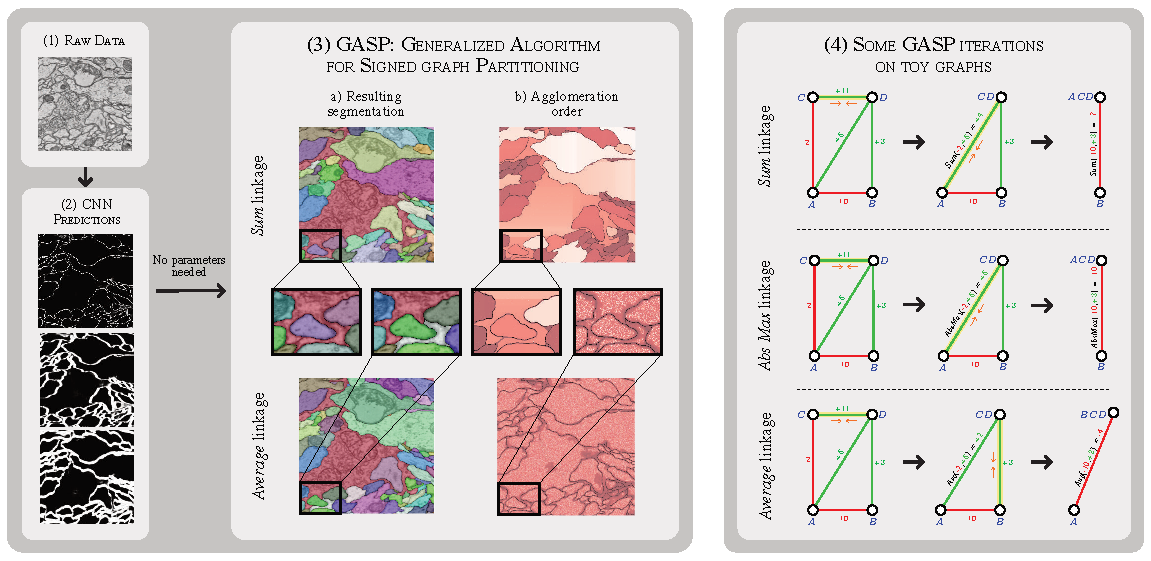
\includegraphics[width=\textwidth]{figs/intro_image_v4.pdf} % left bottom right top
\caption{\algname{} example. \textbf{(1)} Raw data from the CREMI 2016 neuron-segmentation challenge. \textbf{(2)} Some short- and long-range predictions of our CNN model, where white pixels represent boundary evidence. \textbf{(3)} Outputs of two agglomerative algorithms included in our proposed generalized clustering framework, with \emph{Sum} and \emph{Average} linkage criteria. The final clustering / instance segmentation is shown in 3a, overlaid with the raw image.  The  agglomeration order in 3b shows which pairs of neighboring pixels were merged first (white), later on (brown/red), or never (black). (\textbf{4}) Some iterations of \algname{} on toy graph examples with attractive/positive (green) and repulsive/negative (red) interactions. At each iteration, the yellow edge with highest interaction is contracted (orange arrows), until only negative edges are left in the graph. \TODO{Check if avg is correct}
\label{fig:intro_figure}}
\end{figure*}


With our comparison experiments, performed both on 2D urban scenes from the CityScapes dataset and 3D electron microscopy image volumes of neurons, we benchmark all algorithms in our framework, focusing on their efficiency, robustness and tendency to over- or under-cluster.
We show that one of the new algorithms derived from our framework, based on an average linkage criterion, outperforms all previously known agglomeration methods expressed in the framework and that
it achieves competitive performance on CityScapes and the challenging CREMI 2016 segmentation benchmark.

In Sec.~\ref{sec:spectral_clust}, we also show how \algname{} outperforms spectral clustering methods on the task of neuron segmentation and how on synthetic graphs it achieves similar scores to a recently proposed spectral method for signed graphs.

% Our code is available at \url{https://github.com/abailoni/GASP}.



% !TEX root = ../agglo_clust_review.tex

\section{Related work} \label{sec:related_work}
% In recent years there has been considerable progress in pixel-level understanding tasks of computer vision, such as semantic segmentation \cite{long2015fully,kong2018recurrent,chen2018deeplab}, boundary detection \cite{arbelaez2011contour,xie2015holistically,maninis2018convolutional}, %, optical flow \cite{weinzaepfel2013deepflow,dosovitskiy2015flownet},
Recent progress in semantic segmentation \cite{long2015fully,kong2018recurrent,chen2018deeplab}, boundary detection \cite{arbelaez2011contour,xie2015holistically,maninis2018convolutional}, %, optical flow \cite{weinzaepfel2013deepflow,dosovitskiy2015flownet},
and pose estimation \cite{wei2016convolutional,cao2017realtime} was mostly associated with new key ideas and architectures in deep learning, like dilated convolutions \cite{yu2015multi,chen2018deeplab} or ``hourglass'' architectures with skip connections \cite{ronneberger2015u,paszke2016enet} increasing the receptive field of view of the model.

\textbf{Proposal-based methods} decompose the instance segmentation task into two steps that consists in generating object proposals and assigning to each bounding box a class and a binary segmentation mask \cite{he2017mask,yang2012layered,li2017fully,ladicky2010and,hariharan2014simultaneous,chen2015multi,dai2016instance,liang2016reversible}. 
% Here I could have more: \cite{pinheiro2015learning,pinheiro2016learning,hu2017fastmask} and probably something more in Deep coloring
% \item \emph{More references:} or generate generic proposal segments and then label each one with a semantic detector \cite{hariharan2014simultaneous,chen2015multi,hariharan2015hypercolumns,dai2015convolutional,uhrig2016pixel,he2017mask}.
They commonly rely on {Faster-RCNN}~\cite{ren2015faster} and can be trained end-to-end using non-maximum suppression. Other methods use instead recurrent models to sequentially generate instances one-by-one \cite{romera2016recurrent,ren2017end}.

\textbf{Proposal-free methods} adopt a bottom-up approach by directly grouping pixels into instances. For example, the approach proposed in \cite{kirillov2017instancecut} uses a combinatorial framework for joint segmentation; SGN \cite{liu2017sgn} sequentially group pixels into lines and then instances;
% encode instance relationships to classes and exploit the boundary information  \cite{jin2016object}; 
a watershed transform is learned in \cite{bai2017deep} by also predicting its gradient direction, whereas the template matching \cite{uhrig2016pixel} deploys scene depth information.
Others use metric learning to predict high-dimensional associative pixel embeddings that map pixels of the same instance close to each other, while mapping pixels belonging to different instances further apart \cite{fathi2017semantic,newell2017associative,de2017semantic,kulikov2018instance}. % Semi-convolutiona: \cite{novotny2018semi}
% \TODO{What about \cite{liang2018proposal} using spectral clustering?}. 
Final instances are then retrieved by applying a clustering algorithm, like in the end-to-end trainable mean-shift pipeline of \cite{kong2018recurrentPix}.
%  and introducing a fixed number of labels (colors) and then dynamically assigning object instances to those labels during training (coloring) \cite{kulikov2018instance}

\textbf{Edge detection} also experienced recent noticeable progress \cite{xie2015holistically,kokkinos2015pushing}. This is nicely illustrated by the evolution of neuron segmentation for connectomics, a field of neuroscience we also address in our experiments. CNNs were introduced to this application in \cite{jain2007supervised}, but further progress in deep learning and data augmentation lead to much more refined boundary detection \cite{lee2017superhuman,meirovitch2016multi,ciresan2012deep}. 
% or trained an end-to-end watershed region growing algorithm \cite{wolf2017learned}.  
Subsequent postprocessing and superpixel-merging outputs final instances. Some use loopy graphs \cite{kaynig2015large,krasowski2015improving} or trees \cite{meirovitch2016multi,liu2016sshmt,liu2014modular,funke2015learning,uzunbas2016efficient} to represent the region merging hierarchy. The lifted multicut \cite{beier2017multicut} formulates the problem in a combinatorial framework, while flood-filling networks \cite{januszewski2018high} eliminate superpixels by training a recurrent CNN to perform region growing one region at the time. A structured learning approach was also proposed in \cite{funke2018large,turaga2009maximin}.
% \SOURCE{SSHMT} Check Funke proposals

\textbf{Agglomerative graph clustering} has often been applied to instance segmentation \cite{ren2013image,liu2016image,salembier2000binary}, because of its efficiency as compared to other top-down approaches like graph cuts. 
Novel termination criteria and merging strategies have often been proposed: the agglomeration in \cite{malmberg2011generalized} deploys fixed sets of merge constraints; ultrametric contour maps \cite{arbelaez2011contour} combine an oriented watershed transform with an edge detector, so that superpixels are merged until the ultrametric distance exceeds a learned threshold; the popular graph-based method \cite{felzenszwalb2004efficient} stops the agglomeration when the merge costs exceed a measure of quality for the current clusters; whereas the optimization approach in \cite{kiran2014global} performs greedy merge decisions that minimize a certain energy. \TODO{Roman, Cocoons, Benjamin?}
On the other hand, several segmentation pipelines use classical HC linkage criteria, e.g. average linkage \cite{liu2018affinity,lee2017superhuman} or median \cite{funke2018large}. The GALA algorithm in \cite{nunez2013machine,knowles2016rhoananet} features instead a linkage learned by a neural network.

\textbf{Clustering of signed graphs} is another important line of research with the goal of balancing a graph with both attractive and repulsive cues. Finding an optimally balanced clustering has a long history in the field of combinatorial optimization \cite{grotschel1989cutting,grotschel1990facets,chopra1993partition}. %and can be done without the need to specify a termination criterion. 
The name \emph{correlation clustering} was coined by \cite{bansal2004correlation} that also showed its NP-hardness, while its connection with graph multicuts was made by \cite{demaine2006correlation}. Modern integer linear programming solvers can tackle problem instances of considerable size \cite{andres2012globally}, but accurate approximations \cite{pape2017solving,beier2016efficient,yarkony2012fast}, greedy heuristic algorithms \cite{levinkov2017comparative,wolf2018mutex,keuper2015efficient,kardoostsolving} and persistence criteria \cite{lange2018partial,lange2018combinatorial} have been proposed for even larger problems.
\TODO{Cannot-link constraints?}
% Missing: Funke proposals, discussion about cannot-link constraints!!!

\UPDATE{This work combines the clustering algorithms proposed in \cite{levinkov2017comparative,wolf2018mutex,keuper2015efficient} in a simple generalized framework for agglomerative clustering and evaluate them on an instance segmentation task by adopting ideas and CNN architectures from \cite{liu2018affinity,wolf2018mutex,funke2018large} to predict long-range relationships between pixels and boundary evidence between instances.}

% !TEX root = ../agglo_clust_review.tex

\section{Generalized framework for agglomerative clustering of signed graphs} \label{sec:general_framework}
In this section, we first define notation and then introduce one of our main contributions: a signed graph partitioning algorithm (Sec. \ref{sec:algorithm}) that can be seen as a generalization of several existing and new clustering algorithms (Sec. \ref{sec:alg_update_rules}).

\subsection{Notation and graph formalism} \label{sec:notation}

We consider an undirected simple edge-weighted graph $\mathcal{G}(V,E,w^+, w^-)$ with both attractive and repulsive edge attributes. In computer vision applications, the nodes can represent either pixels, superpixels or voxels. We call the set $\Pi$ a \emph{clustering} or \emph{partitioning} with $K$ clusters if $V = \cup_{S\in\Pi} S $, $\,S \cap S' = \emptyset$ for different clusters $S, S'\in \Pi$ and every cluster $S \in \Pi$ induces a connected subgraph of $\mathcal{G}$. We also denote as $S_u$ the cluster associated with node $u$.
The weight function $w^+: E \rightarrow \mathbb{R}^+$ associates to every edge a positive scalar attribute $w_e^+\in \mathbb{R}^+$ representing a merge affinity or a similarity measure: the higher this number, the higher the inclination of the two incident vertices to be assigned to the same cluster\footnote{Note that other formalisms for positively weighted graphs associate distances to the edges, thus, the \emph{lower} the edge weight, the higher the attraction between the two linked nodes, contrary to our definition of $w^+$.}. On the other hand, $w^-: E \rightarrow \mathbb{R}^+$ associates to each edge a split tendency $w_e^- \in \mathbb{R}^+$: the higher this weight, the more the incident vertices would like to be in different clusters. 
Graphs of the type $\mathcal{G}(V,E,w^+, w^-)$ are also often defined as \emph{signed graphs} $\mathcal{G}(V,E,\cost)$, featuring positive and negative edge weights $\cost_e\in \mathbb{R}$. Following the theoretical considerations in \cite{lange2018partial}, we define these signed weights as ${\cost_e = w_e^+ - w_e^-}$. Some approaches directly compute $\cost_e$, whereas others compute $w_e^+$ and $w_e^-$ separately.
In this formalism, graphs with purely attractive interactions are a special case of $\mathcal{G}(V,E,\cost)$ with $\cost_e \geq 0, \, \forall e \in E$.

\textbf{Inter-cluster interaction } We call two clusters $S_u,S_v$ \emph{adjacent} if there exists at least one edge ${e_{ts}\in E}$ connecting a node $t\in S_u$ to a node $s\in S_v$. In hierarchical agglomerative clustering, the interaction $\interact(S_u,S_v)$ between the two clusters is usually defined as a function $\interact{}:\Pi \times \Pi \rightarrow \mathbb{R}$, named \emph{linkage criterion}, depending on the weights of \emph{all} edges connecting clusters $S_u$ and $S_v$, i.e. $(S_u \times S_v) \cap E$. 
All the linkage criteria tested in this article are listed and defined in Table \ref{tab:linkage-criteria}.

\begin{figure}
\centering
        \begin{subfigure}[t]{0.46 \textwidth}
        \centering
        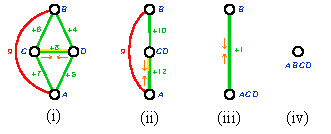
\includegraphics[width=\textwidth]{./figs/example_no_constr.pdf}
        \caption{No constraints}\label{subfig:no_constraints}
    \end{subfigure} \hfill
    \begin{subfigure}[t]{0.46 \textwidth}
        \centering
        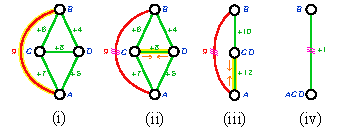
\includegraphics[width=\textwidth]{./figs/example_with_constr.pdf}
        \caption{With cannot-link constraints}\label{subfig:with_constraints}
    \end{subfigure}
\caption{Some iterations of the generalized algorithm (using \emph{Sum} linkage criteria) with and without adding cannot-link constraints. The graph has both attractive (green) and repulsive (red) edges and cannot-link constraints are shown with triple violet bars on the edges. We note that when constraints are enforced, the final clustering is given by two clusters instead of only one.}
\label{fig:algorithm_with_without_CLC}
\end{figure}
\begin{algorithm}[t]
  \caption{\algname{}: generalized algorithm for signed graph partitioning}
   \hspace*{\algorithmicindent} \textbf{Input:} Graph $\mathcal{G}(V,E,w^+,w^-)$; linkage criterion $\interact{}$; boolean {\color{blue}\texttt{addCannotLinkConstraints}}  \\
  \hspace*{\algorithmicindent} \textbf{Output:} Final clustering $\Pi$\\
  \hspace*{\algorithmicindent} 
  \begin{algorithmic}[1]
      \State Initialize clustering $\Pi=\{\{v_1\}, \ldots, \{v_{|V|}\}\}$ with each node in its own cluster
      \State Initial interactions between nodes given by $\cost_e = w^+_e - w^-_e$
      \Repeat
        \State Select pair of clusters $S_u,S_v\in\Pi$ with highest absolute interaction $|\interact{}(S_u,S_v)|$
        \If{\big[{\color{ForestGreen}\textbf{$\interact{}(S_u,S_v) > 0$}}\big] \textbf{and} \big[$S_u,S_v$ are \textbf{not} constrained\big]}
          \State Merge cluster $S_u$ with $S_v$: update interactions and cannot-link constraints with all their neighbors
        \ElsIf{\big[{\color{red}\textbf{$\interact{}(S_u,S_v) \leq 0$}}\big] \textbf{and} {\color{blue}\texttt{addCannotLinkConstraints}}}
          \State Add CannotLink Constraint between clusters $S_u$ and $S_v$
        \EndIf
      \Until{\big[all interactions between clusters are repulsive\big] \textbf{or} \big[all adjacent clusters have cannot-link constraints\big]}
      \State
      \Return $\Pi$
  \end{algorithmic}
  \label{main_alg}
\end{algorithm}

\subsection{\algname{}: generalized algorithm for signed graph partitioning} \label{sec:algorithm} 

In Algorithm \ref{main_alg}, we provide simplified pseudo-code for the proposed \algname{} algorithm. \algname{} implements a bottom-up approach that starts by assigning each node to its own cluster and then iteratively merges pairs of adjacent clusters. The algorithm has two variants. The first one, with \texttt{addCannotLinkConstraints=False}, starts by merging clusters with the strongest attractive interaction and stops once the remaining clusters share only mutual by repulsive interactions (see iterations on toy graphs in block 4 of Fig. \hyperref[fig:intro_figure]{\ref*{fig:intro_figure}}). After each merging iteration, the interaction between the merged cluster and its neighbors is updated according to one of the linkage criteria $\interact(S_u, S_v)$ listed in Table \ref{tab:linkage-criteria}.

In the second variant, when \texttt{addCannotLinkConstraints=True}, Algorithm \ref{main_alg} also introduces \emph{cannot-link constraints}, which represent mutual exclusion relationships between pairs of nodes that cannot be associated with the same cluster in the final clustering. This variant 
selects the pair of clusters with the highest absolute interaction $|\interact(S_u, S_v)|$, so that the most attractive and the most repulsive pairs are analyzed first (see example in Fig. \ref{subfig:with_constraints}). If the interaction is repulsive, then the two clusters are constrained and its members can never merge in subsequent steps. If the interaction is attractive, then the clusters are merged, provided that they were not previously constrained. 
The algorithm terminates when all the remaining clusters are constrained.

In Appendix \ref{sec:detailed_impl}, we comment on the algorithm's computational complexity $\mathcal{O}(N^2 \log N)$ and present our efficient implementation given by the edge contraction Algorithm \ref{detailed_alg} using a priority queue.

\begin{table*}[b]
    \centering
    \scriptsize
    \begin{subtable}[t!]{\textwidth}\centering
        \begin{tabular}{c r  l | c | c  c}
            \multicolumn{3}{c|}{\multirow{2}{*}[-0.5em]{\thead{\textbf{\algname{} linkage criteria} $\,\,\interact(S_u ,S_v)$}}}  & \multirow{2}{*}[-0.5em]{\thead{\textbf{Unsigned Graphs}}} & \multicolumn{2}{c}{\thead{\textbf{Signed Graphs}}}  \\        
            \multicolumn{3}{c|}{} &  &  \multicolumn{1}{c}{\thead{No Constraints}} & \thead{With Constraints} \\        
      
            \midrule
             & Sum: & $\displaystyle \sum_{e\in E_{uv}} \cost_e$ & \thead{Sum Linkage\\Hier. Aggl. Clust.} & \thead{GAEC \cite{keuper2015efficient}} & \thead{Greedy Fixation \cite{levinkov2017comparative}} \\ 
            
             &\makecell[r]{Absolute Max:} & 
            $\displaystyle \cost_e$ with $\displaystyle e = \argmax_{t\in E_{uv}} |\cost_t|$
               & \thead{Single Linkage\\Hier. Aggl. Clust.} & \thead{Mutex Watershed \cite{wolf2018mutex}} & \thead{Mutex Watershed \cite{wolf2018mutex}} \\
             & \makecell[r]{Average:} & $\displaystyle \sum_{e\in E_{uv}} \cost_e \bigg/ \big|E_{uv}\big|  $ & \thead{ Average Linkage\\ Hier. Aggl. Clust.} & \thead{\textbf{NEW}} & \thead{\textbf{NEW}}\\ 

            & Max: & $\displaystyle \max_{e\in E_{uv}} \cost_e$ & \thead{Single Linkage\\Hier. Aggl. Clust.} & \thead{\textbf{NEW}} & \thead{\textbf{NEW}}\\ 

            & Min:& $\displaystyle \min_{e\in E_{uv}} \cost_e$ & \thead{Complete Linkage\\ Hier. Aggl. Clust.}  & \thead{\textbf{NEW}} & \thead{\textbf{NEW}}



            
        \end{tabular}
    \end{subtable} 
    \caption{Existing and new clustering algorithms that can be reformulated as special cases of the proposed generalized algorithm for signed graph partitioning \algname{}, given a linkage criterium, a type of graph (signed or unsigned) and the optional use of cannot-link constraints. The set $E_{uv}$ is defined as the set of all edges connecting cluster $S_u$ to cluster $S_v$, i.e. $E_{uv}=(S_u \times S_{v \neq u}) \cap E$.}
    \label{tab:linkage-criteria}
\end{table*}
\begin{figure}
\centering
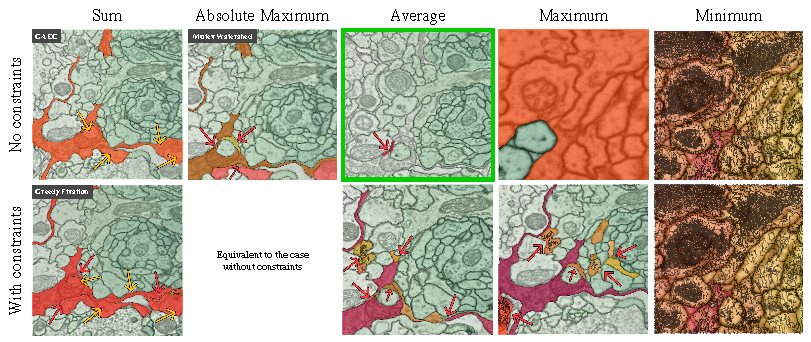
\includegraphics[width=\textwidth]{./figs/comparison_new.pdf} % left bottom right top
\caption{Failure cases of \algname{} with different linkage criteria highlighted on some difficult parts of the CREMI Challenge data. The main \emph{wrongly} segmented regions are highlighted in different warm colors. Note that the data is 3D, hence the same color could be assigned to parts of segments that appear disconnected in 2D.  Red arrows point to wrongly split regions. Yellow arrows point out merge errors. The \emph{Average} linkage without cannot-link constraints returned the best segmentation.
\label{fig:cremi_comparison}}
\end{figure}



\subsection{\algname{} with different linkage criteria: new and existing algorithms} \label{sec:alg_update_rules}

Our main contribution is the generalized algorithm for signed graph partitioning, short GASP, that encompasses several known and novel agglomerative algorithms on display in Table \ref{tab:linkage-criteria}.
In our framework, individual algorithms are differentiated by the linkage criterion employed. We review them in the following paragraphs.

In the special case of an unsigned graph with only positive interactions, i.e. $w_e^-=0$ and $\cost_e \geq 0$ $\forall e\in E$, 
 the algorithm performs a standard agglomerative hierarchical clustering by returning only a single cluster and a hierarchy of clusters defined by the order in which the clusters are merged (see Table \ref{tab:linkage-criteria}, unsigned graphs).

Given a graph with both attractive and repulsive cues, an edge contraction algorithm with a sum update rule was pioneered in \cite{levinkov2017comparative,keuper2015efficient} (Table \ref{tab:linkage-criteria}, \emph{Sum} linkage). The authors present both a version with cannot-link constraints and one without, and then compare them with other greedy local-search algorithms approximating the multicut optimization problem.
The Mutex Watershed \cite{wolf2018mutex} is another signed graph partitioning algorithm that introduces dynamical cannot-link constraints. In Proposition \ref{prop:equiv_MWS} (see Appendix \ref{sec:appendix_abs_max}) we prove that, surprisingly, it can also be seen as an efficient implementation of \algname{} with \emph{Absolute maximum} linkage (see def. in Table \ref{tab:linkage-criteria}). Moreover, in Proposition \ref{prop:abs_max_cannot_link_property} we also prove that \algname{} with \emph{Abs Max} linkage returns the same clustering with or without enforcing cannot-link constraints.
On the other hand, to our knowledge, \emph{Average}, \emph{Max} or \emph{Min} linkage criteria have never been used for signed graph agglomerative algorithms or been combined with cannot-link constraints.

Apart from the linkage criteria defined in Table \ref{tab:linkage-criteria}, additional ones were proposed in the literature:
\cite{nunez2013machine} for example uses a learned approach where a random forest classifier updates the cluster interactions depending on predefined edge and node features; other approaches introduce a weight regularization depending on the size of the clusters \cite{felzenszwalb2004efficient,kardoostsolving}, whereas 
\cite{funke2018large} uses a \emph{quantile} linkage criteria by populating a histogram for each inter-cluster interaction. In our experiments, we decided to focus on the linkage criteria listed in Table \ref{tab:linkage-criteria}, since they represent the most common options.


% !TEX root = ../agglo_clust_review.tex
\section{Experiments on neuron segmentation}

We first evaluate and compare the agglomerative clustering algorithms described in the generalized framework on the task of neuron segmentation in electron microscopy (EM) image volumes. This application is of key interest in connectomics, a field of neuro-science with the goal of reconstructing neural wiring diagrams spanning complete central nervous systems. While a lot of progress is being made, only proof-reading or manual tracing yields sufficient accuracy for correct circuit reconstruction \cite{schlegel2017learning}.
\TODO{subsections description}

\subsection{Experimental setup and pixel grid-graph} \label{sec:grid_graph}
EM segmentation is commonly performed by first predicting which pixels belong to a cell membrane using a CNN and then applying 

\begin{itemize}
\item Define predictions of the classifier (pseudo probabilities) for edge weights
\item Define possible mappings to signed costs
\item Make comment about which version defines nested segmentations and which does not give hirarchical solutions

\end{itemize}


\begin{itemize}
    \item Define long-range grid graph. (Mention the fact of enforcing local merge)
\item Introduce "Poisson" random graph with a given probability of long-range connections
\item Comment about the short- and long-range distinction in the MWS paper? It does not work that well in practice (applying post-processing to remove small segments is easier and better solution).
\item Ad of course we can think about a classifier that separately predict attraction and repulsion
\item Define offset patterns (link to supplementary material), trained networks (loss, etc...) and setups on cremi and cityscapes 
\item Mention postprocessing step: get rid of tiny segments; on CREMI we use watershed to fill the deleted parts 
\end{itemize}

% !TEX root = ../agglo_clust_review.tex


\begin{figure}[t]
\centering
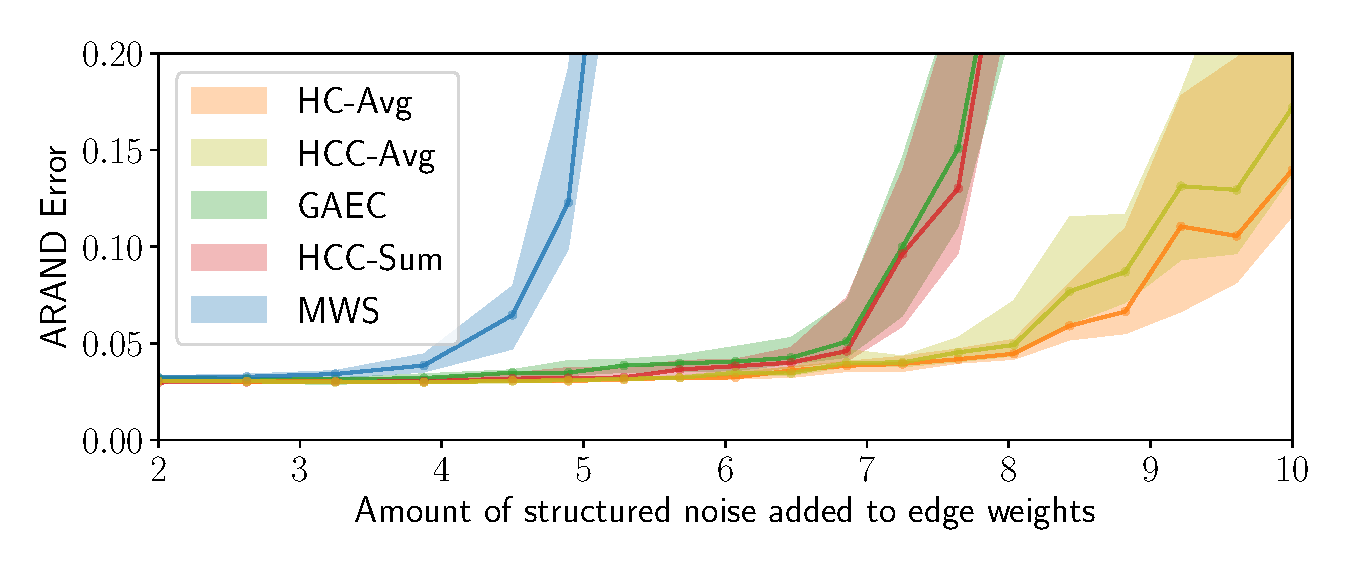
\includegraphics[width=0.47\textwidth,trim=0.2in 0.17in 0.2in 0.2in,clip]{./figs/noise_plots/noise_plots_adapted-rand_1.pdf}
        \caption{
ARAND errors (median values over 20 experiments, lower is better) on \emph{CREMI-gridGraph} clustering problems perturbed with structured noise. Average-linkage algorithms proved to be the most robust.
% We report median, 25th, and the 75th percentile values over \TODO{30} experiments.
% \algname{} performances compared to spectral methods on synthetic graphs. The spectral methods were given the true number of clusters as input, in contrast to \algname{}. \TODO{Define paramters SSB; explain percentile stuff (for both noise experiments), user ARAND-error}
}\label{fig:scores_structured_noise}
\end{figure}

% \captionsetup[subfigure]{justification=centering, singlelinecheck=off}
% \begin{figure}[t]
% \centering
%     \begin{subfigure}[t]{0.47 \textwidth}
%         \centering
%         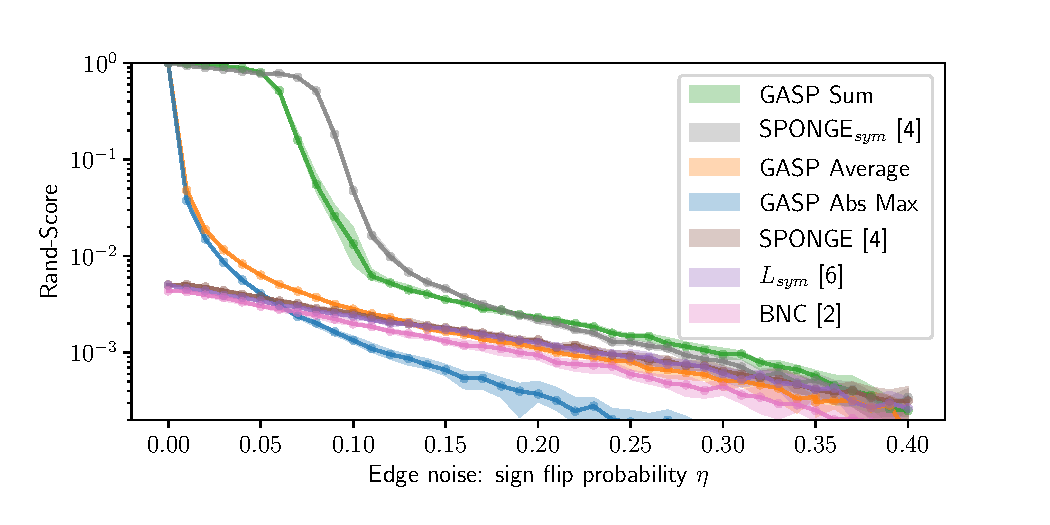
\includegraphics[width=\textwidth,trim=0.25in 0.in 0.5in 0.in,clip]{./figs/SSBM_experiments.pdf}
%         \caption{Scores on SSBM graphs}
%     \end{subfigure} \hfill
%     \begin{subfigure}[t]{0.47 \textwidth}
%         \centering
%         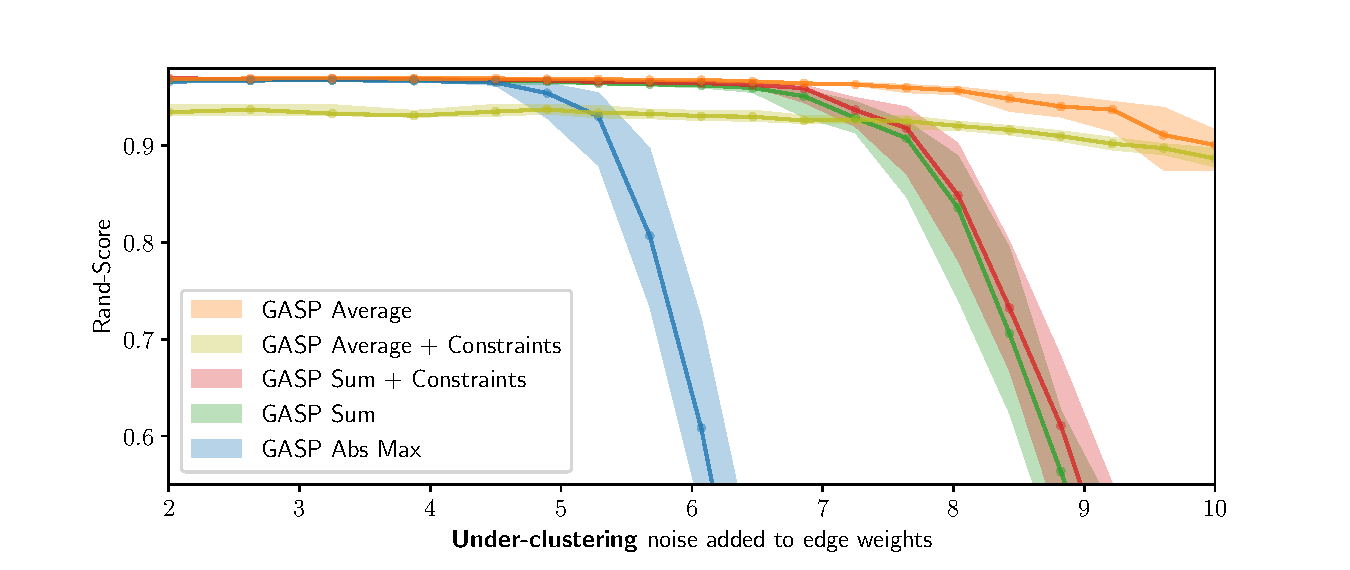
\includegraphics[width=\textwidth,trim=0.53in 0.1in 0.65in 0.45in,clip]{./figs/noise_plots/under_segment_plots_1.pdf}
%         \caption{Scores on \emph{CREMI-gridGraph} perturbed with noise}
%     \end{subfigure}

%     % \begin{subfigure}[t]{0.32 \textwidth}
%     %     \centering
%     %     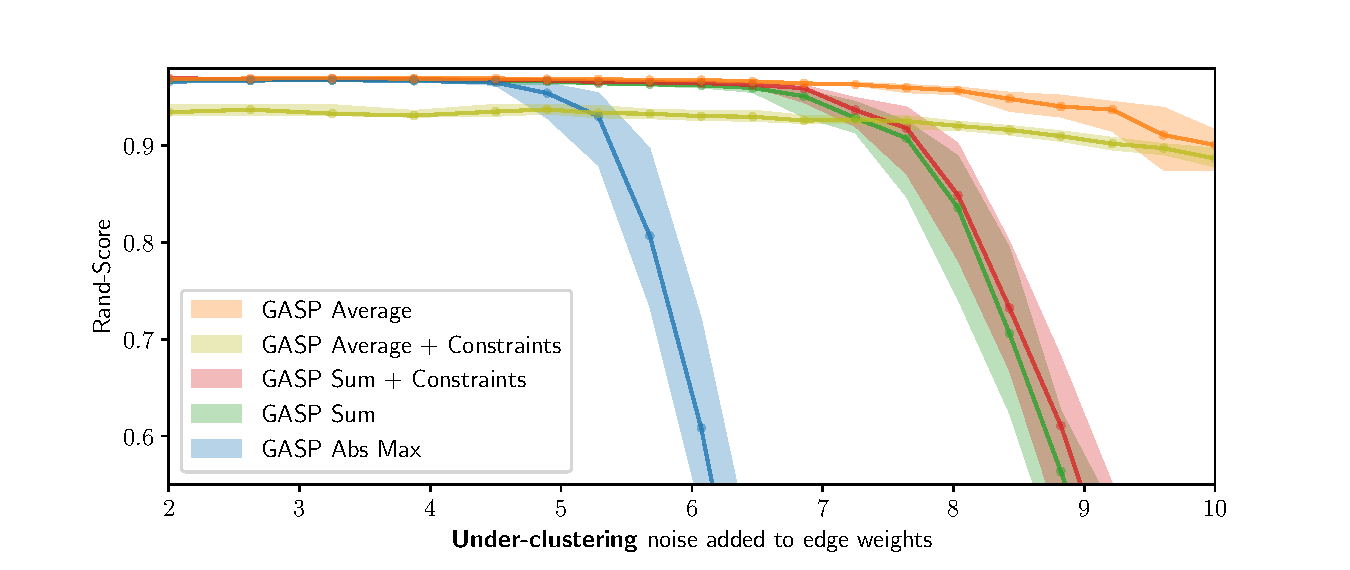
\includegraphics[width=\textwidth,trim=0.53in 0.1in 0.65in 0.45in,clip]{./figs/noise_plots/under_segment_plots_1.pdf}
%     % \end{subfigure}\hfill
%     % \begin{subfigure}[t]{0.32 \textwidth}
%     %     \centering
%     %     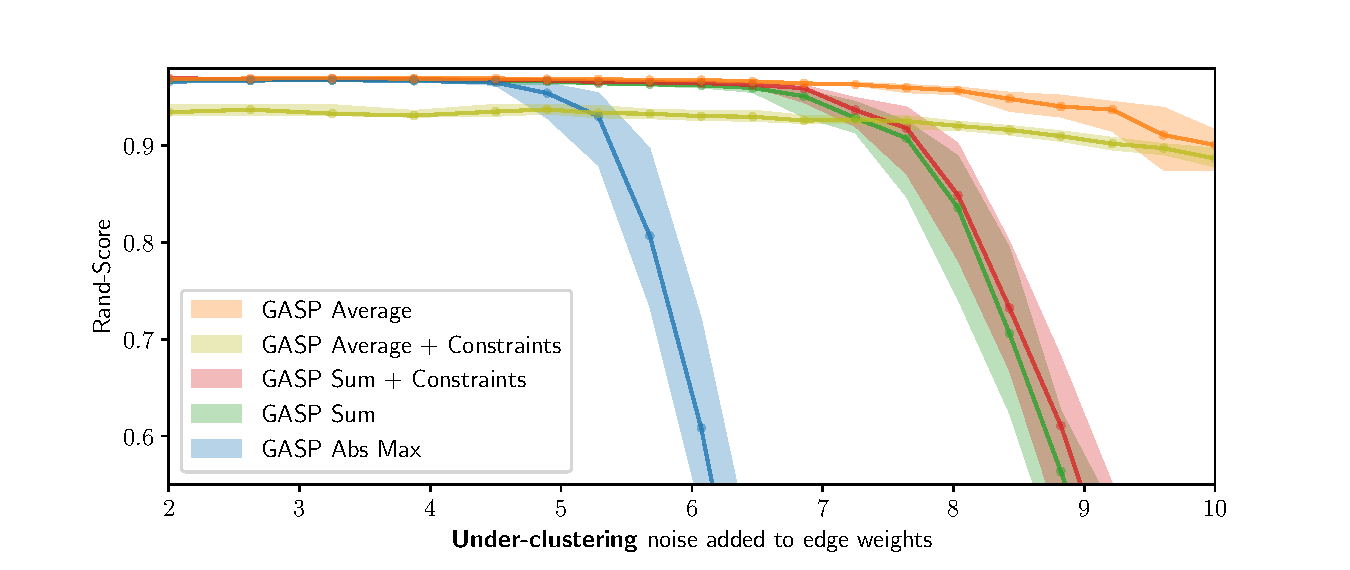
\includegraphics[width=\textwidth,trim=0.53in 0.1in 0.65in 0.45in,clip]{./figs/noise_plots/under_segment_plots_1.pdf}
%     % \end{subfigure}
%     %     \begin{subfigure}[t]{0.49 \textwidth}
%     %     \centering
%     %     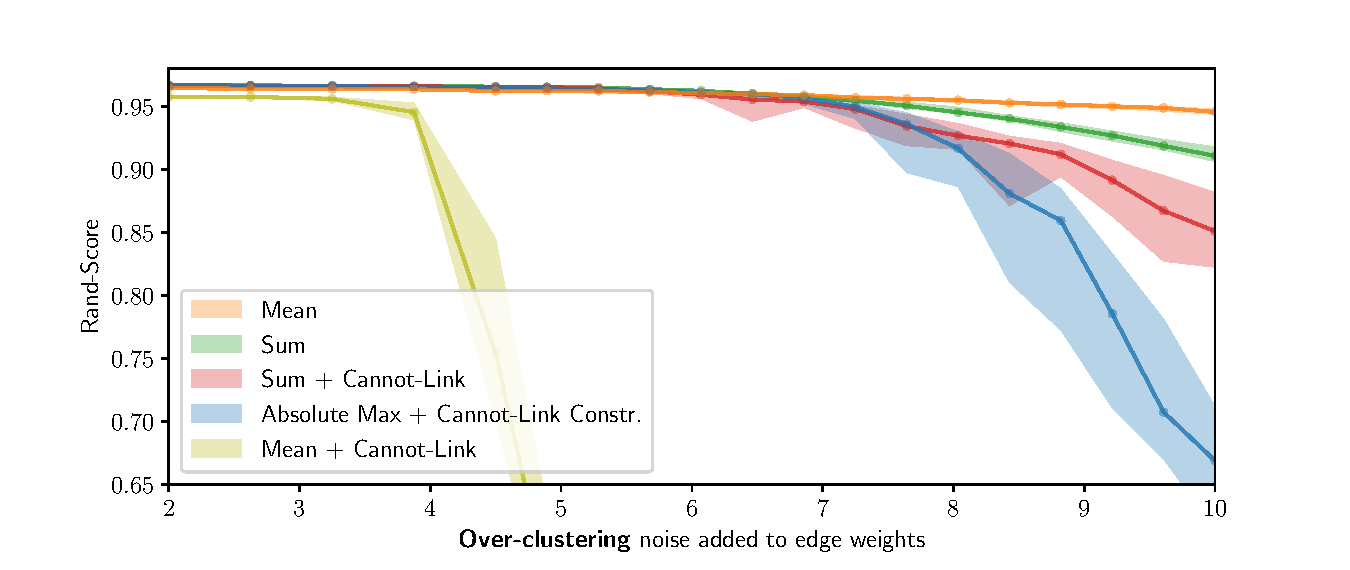
\includegraphics[width=\textwidth,trim=0.53in 0.1in 0.65in 0.45in,clip]{./figs/noise_plots/over_segment_plots_0.pdf}
%     %     \caption{No long-range predictions: \\$p_{\mathrm{long}}=0$} \label{fig:merge_noise_only_direct}
%     % \end{subfigure} \hfill
%     % \begin{subfigure}[t]{0.49 \textwidth}
%     %     \centering
%     %     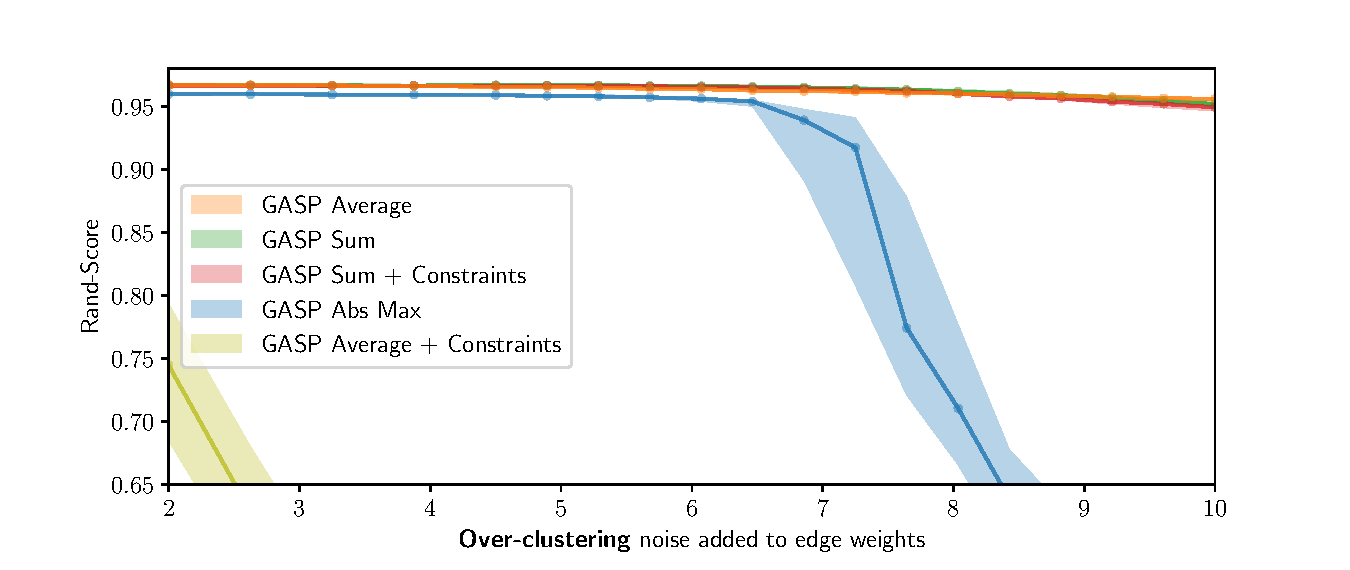
\includegraphics[width=\textwidth,trim=0.53in 0.1in 0.65in 0.45in,clip]{./figs/noise_plots/over_segment_plots_1.pdf}
%     %     \caption{With long-range predictions: $p_{\mathrm{long}}=0.1$} \label{fig:merge_noise_with_long_range}
%     % \end{subfigure}
% \caption{\algname{} sensitivity to noise: \emph{Average} linkage proved to be the most robust. Performances are given by Rand-Score (higher is better) depending on the amount of noise added to the CNN predictions. Solid lines represent median values over 30 experiments. Values between the 25th and the 75th percentile are shown in shaded areas. The two sets of experiments using under- and over-clustering noise are summarized in the plots at the top and at the bottom, respectively (see Appendix \ref{sec:appendix_noise_gen} for more details). For each experiment, some of the long-range CNN predictions were randomly selected with probability $p_{\mathrm{long}}$ and added as long-range edges to the pixel grid-graph. Experiments are performed on a crop of CREMI training sample B.
% \algname{} performances compared to spectral methods on synthetic graphs. The spectral methods were given the true number of clusters as input, in contrast to \algname{}. \TODO{Define paramters SSB; explain percentile stuff (for both noise experiments), user ARAND-error}
% }\label{fig:noise_plots}
% \end{figure}


% \begin{figure}[t]
% \centering
% % \begin{minipage}[t]{0.48\textwidth}
% % \vspace{0pt}
% % \centering
% % % \footnotesize
% % \begin{tabular}[t]{L{9em} M{7em}}
% %            Method & Rand-Score \\ \midrule
% %            \textbf{GASP Average} & \textbf{0.8966} \\
% % GASP Sum & 0.8965 \\
% % GASP Abs Max & 0.8932 \\
% % SPONGE$_{sym}$ \cite{Cucuringu2019SPONGEAG} & 0.5839\\
% % $L_{sym}$ \cite{kunegis2010spectral} & 0.1931 \\
% % SPONGE \cite{Cucuringu2019SPONGEAG} & 0.0789 \\
% % BNC \cite{chiang2012scalable} & 0.0074 \\
% %         \end{tabular}
% %     \captionof{table}{\algname{} compared to spectral clustering methods on a small crop of the CREMI dataset (sample B).}
% %     \label{tab:cremi_spectral_experiments}
% % \end{minipage}\\\vspace{2em}
% \begin{minipage}[t]{0.38\textwidth}
% \vspace{0pt}
% \centering
%         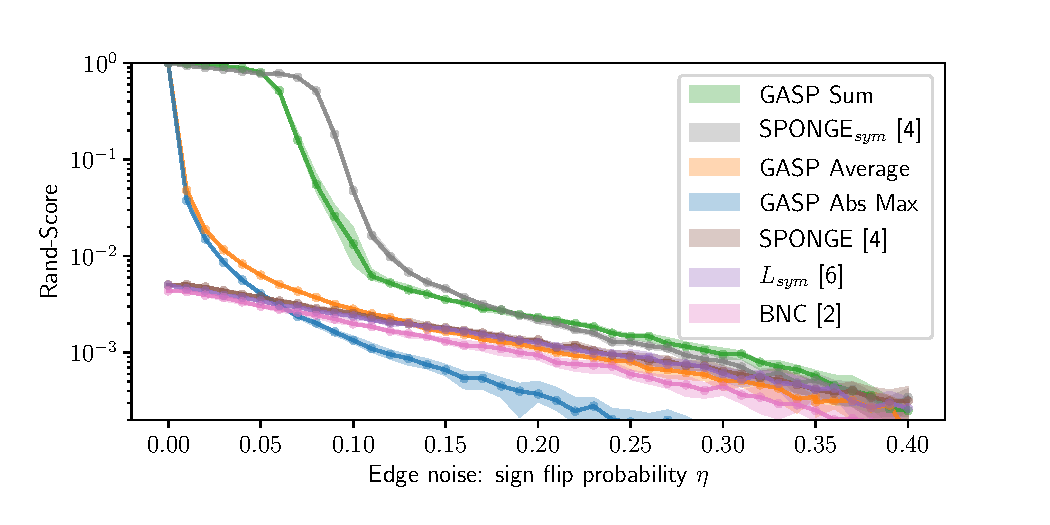
\includegraphics[width=1.\textwidth,trim=0.25in 0.25in 0.68in 0.36in,clip]{./figs/SSBM_experiments.pdf} % 0.45
%         \caption{}
%     \label{fig:SSBM_scores}
% \end{minipage}
% \end{figure}






% \subsection{Data: CREMI challenge} \label{sec:cremi_challenge}
% Test \ref{tab:cremi_leaderboard}
% We evaluate all algorithms in the proposed framework on the competitive CREMI 2016 EM Segmentation Challenge \cite{cremiChallenge} that is currently the neuron segmentation challenge with the largest amount of training data available. The dataset comes from serial section EM of \emph{Drosophila} fruit-fly tissue and consists of 6 volumes of 1250x1250x125 voxels at resolution 4x4x40nm, three of which come with publicly available training ground truth. The results submitted to the leaderboard are evaluated using the CREMI score, based on the Adapted Rand-Score (Rand-Score) and the Variation of Information Score \cite{arganda2015crowdsourcing}. In Appendix \ref{sec:cremi_details}, we provide more details about the training of our CNN model, inspired by work of \cite{lee2017superhuman,funke2018large}.

% !TEX root = ../agglo_clust_review.tex


\subsection{Results and discussion}\label{sec:results}
\textbf{Comparison of linkage criteria} Table \ref{tab:results_cremi_train} shows how the agglomerative algorithms derived from our framework compare to each other. For a simple baseline, we also include a segmentation produced by thresholding the affinity predictions (THRESH).
\algname{} with \emph{Average} linkage, representing one of the new algorithms derived from our generalized framework, significantly outperformed all other previously proposed agglomerative methods like GAEC (\algname{} Sum) \cite{keuper2015efficient}, Greedy Fixation (\algname{} Sum + Constraints) \cite{levinkov2017comparative} or Mutex Watershed (\algname{} Abs. Max.) \cite{wolf2018mutex}. The competitive performance of this simple parameter-free algorithm is also reported in Table \ref{tab:results_cremi_test}, showing the current leader-board of the challenge: all entries, apart from \algname{}, employ superpixel-based post-processing pipelines, several of which rely on the lifted multicut formulation of \cite{beier2017multicut} that uses several random forests to predict graph edge weights, relying not only on information derived from affinity maps but also raw data and shape information.
Note that the test volumes contain several imaging artifacts that make segmentation particularly challenging and might profit from more robust edge statistics of super-pixel based approaches.
On the other hand, the fact that our algorithm can operate on pixels directly removes the parameter tuning necessary to obtain good super-pixels and can also avoid errors that result from wrong superpixels that cannot be fixed during later agglomeration.
In Appendix \ref{sec:appendix_exps_full_cremi}, we provide more details about how we scaled up \algname{} to the full datasets. Appendix Table \ref{tab:extended_results_cremi} lists the performances and the run-times for all tested \algname{} linkage.


\begin{figure}[t]
        \centering
\begin{minipage}[t]{0.56\textwidth}
    \centering
    \scriptsize
        \begin{tabular}[t]{l|c}
          & \makecell{CREMI-Score \\(lower is better)} \\ \midrule 
\textbf{\algname{}} \textbf{Average}& \textbf{0.226}  \\
\algname{} Sum + Constraints \cite{levinkov2017comparative} & 0.282 \\
\algname{} Abs. Max. \cite{wolf2018mutex} & 0.322 \\
\algname{} Max. + Constraints & 0.324 \\
\algname{} Sum \cite{keuper2015efficient} & 0.334 \\
\algname{} Average + Constraints & 0.563 \\
THRESH & 1.521 \\ 
        \end{tabular}
    \captionof{table}{CREMI-Scores achieved by different linkage criteria and thresholding. All methods use the affinity predictions from our CNN as input. Scores are averages over the three CREMI training datasets.}
    \label{tab:results_cremi_train}
\end{minipage}\hfill
\begin{minipage}[t]{0.4\textwidth}
    \centering
    \scriptsize
        \begin{tabular}[t]{l|c}
         & \makecell{CREMI-Score \\(lower is better)}  \\ \midrule
Our CNN + DTWS + LMC &  0.221\\
PNI CNN \cite{lee2017superhuman} & 0.228 \\
\textbf{Our CNN + \algname{} Average} & \textbf{0.241} \\
MALA CNN + MC \cite{funke2018large} & 0.276 \\
CRU-Net \cite{zeng2017deepem3d} & 0.566  \\
LFC \cite{parag2017anisotropic} & 0.616  \\
        \end{tabular}
        \vspace*{1em}
    \captionof{table}{Current leading entries  in the CREMI challenge leaderboard \cite{cremiChallenge} (May 2019). The scores are averages of the three test datasets.}
    \label{tab:results_cremi_test}
\end{minipage}
\end{figure}
\captionsetup[subfigure]{justification=centering, singlelinecheck=off}
\begin{figure}
\centering
    \begin{subfigure}[t]{0.49 \textwidth}
        \centering
        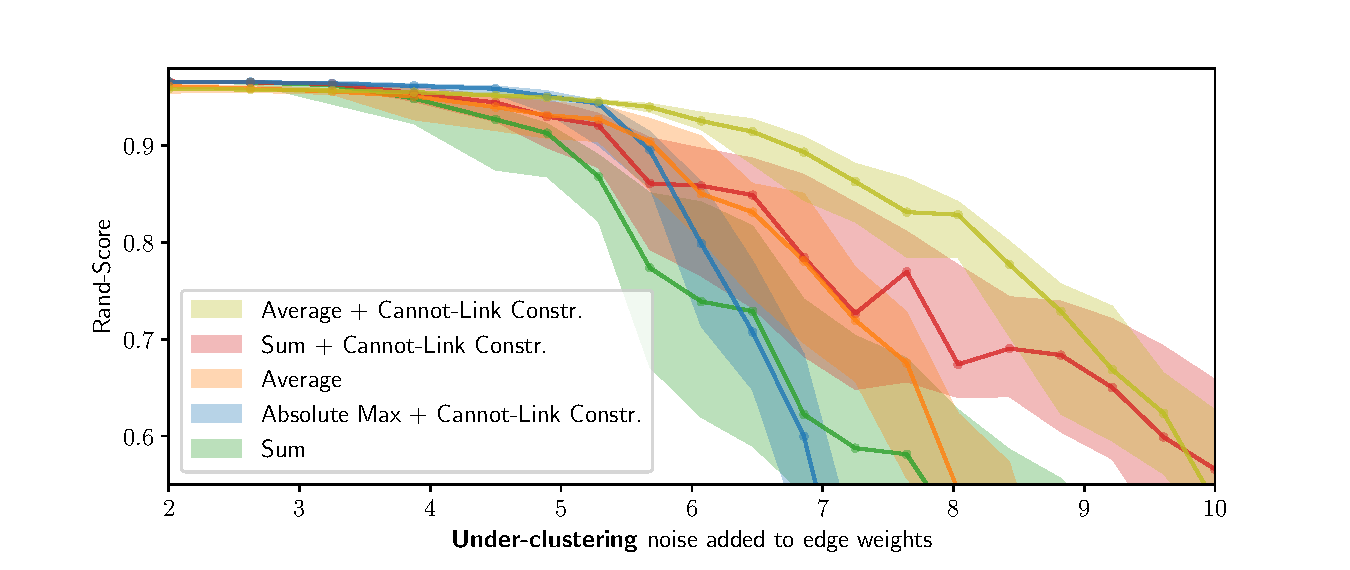
\includegraphics[width=\textwidth,trim=0.55in 0.1in 0.65in 0.45in,clip]{./figs/noise_plots/under_segment_plots_0.pdf}
    \end{subfigure} \hfill
    \begin{subfigure}[t]{0.49 \textwidth}
        \centering
        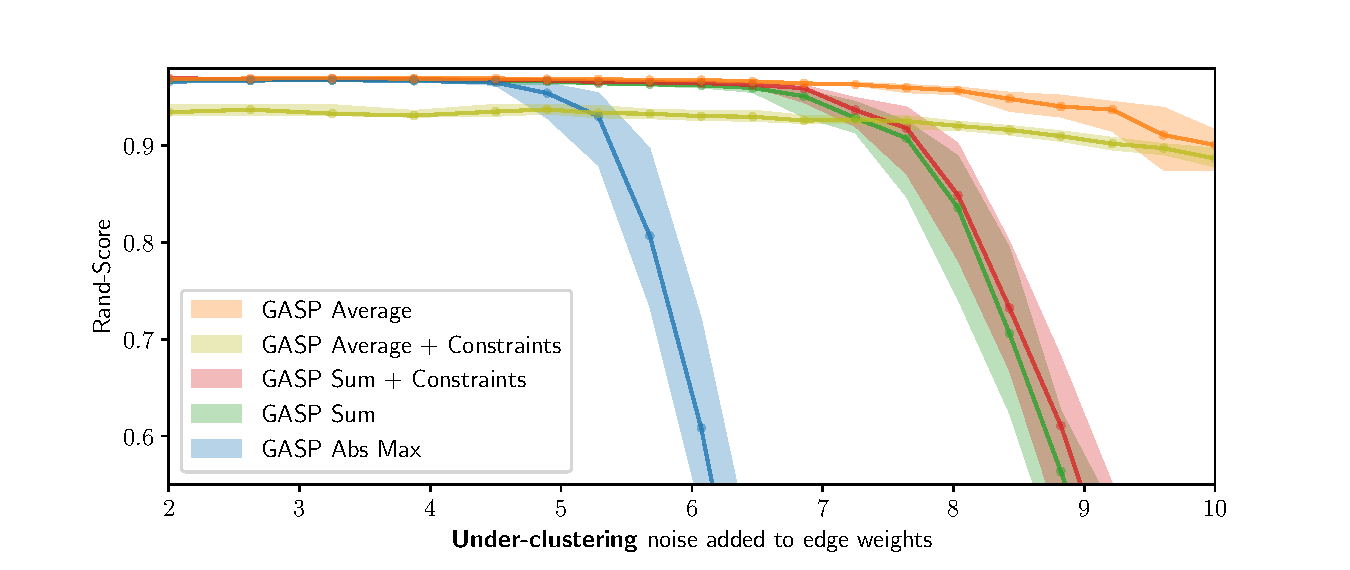
\includegraphics[width=\textwidth,trim=0.53in 0.1in 0.65in 0.45in,clip]{./figs/noise_plots/under_segment_plots_1.pdf}
    \end{subfigure}

        \begin{subfigure}[t]{0.49 \textwidth}
        \centering
        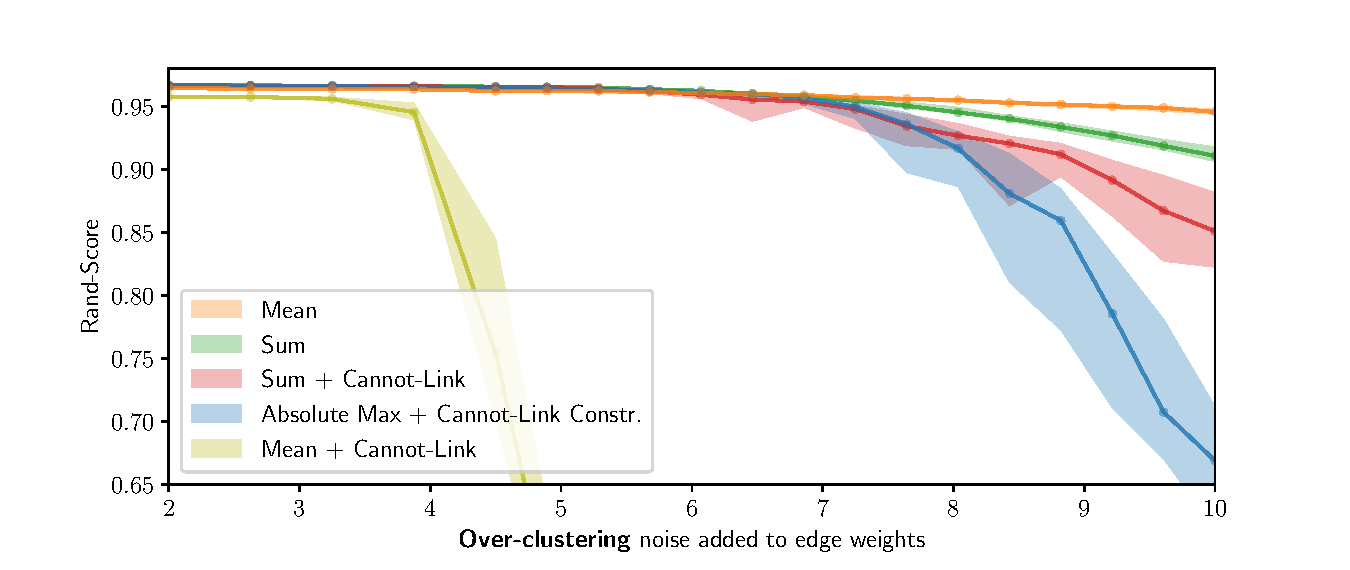
\includegraphics[width=\textwidth,trim=0.53in 0.1in 0.65in 0.45in,clip]{./figs/noise_plots/over_segment_plots_0.pdf}
        \caption{No long-range predictions: $p_{\mathrm{long}}=0$} \label{fig:merge_noise_only_direct}
    \end{subfigure} \hfill
    \begin{subfigure}[t]{0.49 \textwidth}
        \centering
        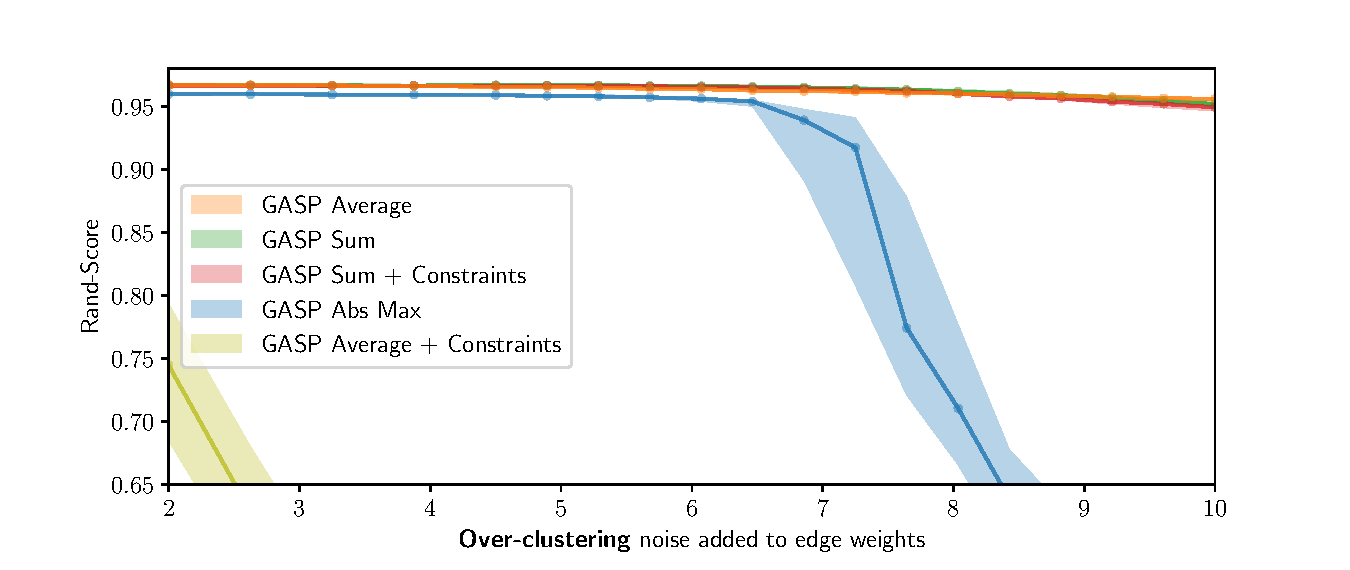
\includegraphics[width=\textwidth,trim=0.53in 0.1in 0.65in 0.45in,clip]{./figs/noise_plots/over_segment_plots_1.pdf}
        \caption{With long-range predictions: $p_{\mathrm{long}}=0.1$} \label{fig:merge_noise_with_long_range}
    \end{subfigure}
\caption{\algname{} sensitivity to noise: \emph{Average} linkage proved to be the most robust. Performances are given by Rand-Score (higher is better) depending on the amount of noise added to the CNN predictions. Solid lines represent median values over 30 experiments. Values between the 25th and the 75th percentile are shown in shaded areas. The two sets of experiments using under- and over-clustering noise are summarized in the plots at the top and at the bottom, respectively (see Appendix \ref{sec:appendix_noise_gen} for more details). For each experiment, some of the long-range CNN predictions were randomly selected with probability $p_{\mathrm{long}}$ and added as long-range edges to the pixel grid-graph.
}\label{fig:noise_plots}
\end{figure}


\textbf{Noise experiments }  Additionally, we conduct a set of experiments where the CNN predictions are perturbed by structured noise, in order to highlight the properties of each \algname{} variant and perform an in-depth comparison that is as quantitative as possible. Appendix \ref{sec:appendix_noise_gen} introduces the type of spatially correlated noise that allowed us to perturb the CNN outputs by introducing simulated additional artifacts like missing or false positive boundary evidence. 
Fig. \ref{fig:noise_plots} summarizes our 12000 noise experiments: we focus on the best performing linkage criteria, i.e. \emph{Average}, \emph{Sum} and \emph{Abs Max}, and test them with different amount of noise. 
In these experiments, we also want to assess how beneficial it is to use long-range CNN predictions in the agglomeration. Thus, we perform a set of simulations without adding long-range connections to the grid-graph and another set where we introduce them with a 10\% probability\footnote{We also performed experiments adding all the long-range predictions given by the CNN model, but we did not note major differences when using only 10\% of them. Adding this fraction is usually sufficient to improve the scores.}.

\textbf{Average and Abs Max linkage } Our findings confirm that \algname{} with \emph{Average} linkage criterion represents the most robust algorithm tested and the one that benefits the most from using the long-range CNN predictions. On the other hand, it is not a surprise that the \emph{Abs Max} statistic proposed by \cite{wolf2018mutex} is less robust to noise than the \emph{Average} linkage, but, as we show in the Appendix Table \ref{tab:extended_results_cremi}, \emph{Abs Max} represents a valid and considerably faster option. 
Adding long-range connections to the graph is generally helpful, but when many of them carry repulsive weights, then \algname{} with cannot-link constraints shows a clear tendency to over-cluster.    

\textbf{Sum linkage } 
All our experiments show that \algname{} with \emph{Sum} linkage is the algorithm with the highest tendency to under-cluster and incorrectly merge segments (see Fig. \ref{fig:cremi_comparison} for an example). This property is related to the empirical observation that a \emph{Sum} statistic tends to grow clusters one after the other, as shown in Fig. \ref{fig:intro_figure} by the quite unique agglomeration order of the \emph{Sum} statistic. An intuitive explanation of this fact is the following: initially, most of the intra-cluster nodes present similar attractive interactions between each others; when the two nodes sharing the most attractive interaction are merged, there is a high chance that they both share an attractive interaction with a common neighboring node, so the new interaction with this common neighbor will be immediately assigned to a high priority in the agglomeration, given by the sum of two high weights; this usually starts a ``chain reaction'', where only a single cluster is agglomerated at the beginning. On the other hand, as we also see in Fig. \ref{fig:intro_figure}, other linkage criteria like \emph{Average} or \emph{Abs Max} grow clusters of similar sizes in parallel and accumulate in this way much more reliable inter-cluster statistics.






% !TEX root = ../agglo_clust_review.tex
\subsection{Scores on CREMI challenge}

% % !TEX root = ../agglo_clust_review.tex
\section{Experiments on CityScapes}\label{sec:cityscapes_exp}
We also evaluate the performances of \algname{} on the CityScapes dataset \cite{cordts2016cityscapes}, which consists of 5000 street-scene images: 2975 for training, 500 for validation and 1525 for testing.
% recorded by car-mounted cameras with resolution 1024$\times$2048: 2975 images for training, 500 for validation and 1525 for testing. Objects with instance-level annotations belong to the following classes: person, rider, car, truck, bus, train, motorcycle, bicycle. 
For our experiments, we used the state-of-the-art proposal-free pipeline proposed in GMIS \cite{liu2018affinity} that achieved superior performances compared to other proposal-based methods like Mark R-CNN and employs a similar model to the one applied by us on neuron-segmentation.
Their trained model was made publicly available, so we simply replaced their final graph-merging algorithm (MultiStepHAC) with \algname{}. See Appendix \ref{sec:appendix_cityscapes} for more details on how we fine-tuned their instance branch model by using a \emph{S\o resen-Dice} loss similarly to \cite{wolf2018mutex} and obtained in this way sharper affinity-predictions.

Results are summarized in Table \ref{tab:results_cityscapes_val} and confirm our findings on neuron-segmentation: \algname{} with average linkage achieves the best scores, whereas other linkage tend to introduce more false region-splits, like \emph{Abs. Max.}, or false region-merge, like \emph{Sum}. In Appendix, Table \ref{tab:extended_results_cityscapes_val} includes all other tested linkage. MultiStepHAC requires the user to tune several threshold parameters and it was probably tailored to the original affinities predicted by \cite{liu2018affinity}, so it did not generalize well to our fine-tuned model and it achieved lower scores compared to the original AP value of 34.1 reported in \cite{liu2018affinity}.  


\begin{figure}[t]
\centering
\begin{minipage}[T]{0.59\textwidth}
    \centering
    \footnotesize
        \begin{tabular}{l|l|cc}
           & Agglomeration  &  \multicolumn{2}{c}{Use constraints:} \\
          Pipeline & method & \textsc{No} & \textsc{Yes} \\ \midrule
DWT \cite{bai2017deep} & - & 21.2 & - \\
SGN \cite{liu2017sgn} & - & 29.2 & - \\
Mask RCNN \cite{he2017mask} & - & 31.5 & - \\ \hline
 & \textbf{\algname{} Average}& \textbf{34.3}  & 33.9  \\
\multirow{2}{*}{GMIS \cite{liu2018affinity}} & MultiStepHAC \cite{liu2018affinity} & \UPDATE{33.0} & -  \\
 % & \algname{} Max &   24.3  &   32.5  \\
 & \algname{} Abs. Max. \cite{wolf2018mutex}  & 32.1 & 32.1 \\
 & \algname{} Sum \cite{keuper2015efficient,levinkov2017comparative} & 31.3  & 31.9  \\
 % & \algname{} Min &  0    & 0  \\
        \end{tabular}
    \captionof{table}{Average Precision (AP) scores on the cityscapes validation set achieved by the tested pipelines}
    \label{tab:results_cityscapes_val}
\end{minipage}\hfill
\begin{minipage}[T]{0.37\textwidth}
    \centering
\includegraphics[width=\textwidth]{./figs/cityscapes_compare_2.pdf} % left bottom right top
\end{minipage}
\end{figure}

% !TEX root = ../agglo_clust_review.tex



% \begin{figure*}[htp]
% \captionsetup{font=small}
% \hspace*{\fill}
% \begin{minipage}[t]{0.38\textwidth}
% \centering
% \vspace{0pt}
%         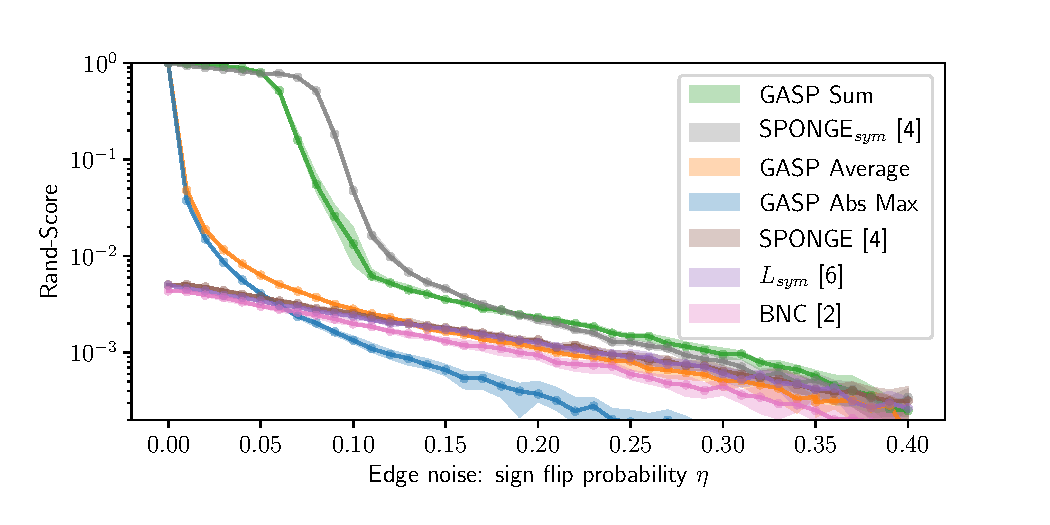
\includegraphics[width=\textwidth,trim=0.25in 0.25in 0.68in 0.36in,clip]{./figs/SSBM_experiments.pdf}
%         \captionof{figure}{Experiments on SSBM synthetic graphs}
%     \label{fig:SSBM_experiments}
% \end{minipage}\hfill
% \begin{minipage}[t]{0.25\textwidth}
% \centering
% \vspace{0pt}
%     \scriptsize
% \begin{tabular}{l|c}
%            Method & Rand-Score \\ \midrule
%            \textbf{GASP Average} & \textbf{0.8966} \\
% GASP Sum & 0.8965 \\
% GASP Abs Max & 0.8932 \\
% SPONGE$_{sym}$ \cite{Cucuringu2019SPONGEAG} & 0.5839\\
% $L_{sym}$ \cite{kunegis2010spectral} & 0.1931 \\
% SPONGE \cite{Cucuringu2019SPONGEAG} & 0.0789 \\
% BNC \cite{chiang2012scalable} & 0.0074 \\
%         \end{tabular}
%     \captionof{table}{Experiments on a tiny crop of the CREMI dataset, training sample B.}
%     \label{tab:cremi_experiments}
% \end{minipage}
% \end{figure*}

\begin{figure}[t]
\centering
\begin{minipage}[t]{0.48\textwidth}
\vspace{0pt}
\centering
% \footnotesize
\begin{tabular}[t]{L{9em} M{7em}}
           Method & Rand-Score \\ \midrule
           \textbf{GASP Average} & \textbf{0.8966} \\
GASP Sum & 0.8965 \\
GASP Abs Max & 0.8932 \\
SPONGE$_{sym}$ \cite{Cucuringu2019SPONGEAG} & 0.5839\\
$L_{sym}$ \cite{kunegis2010spectral} & 0.1931 \\
SPONGE \cite{Cucuringu2019SPONGEAG} & 0.0789 \\
BNC \cite{chiang2012scalable} & 0.0074 \\
        \end{tabular}
    \captionof{table}{\algname{} compared to spectral clustering methods on a small crop of the CREMI dataset (sample B).}
    \label{tab:cremi_spectral_experiments}
\end{minipage}\\\vspace{2em}
\begin{minipage}[t]{0.48\textwidth}
\vspace{0pt}
\centering
        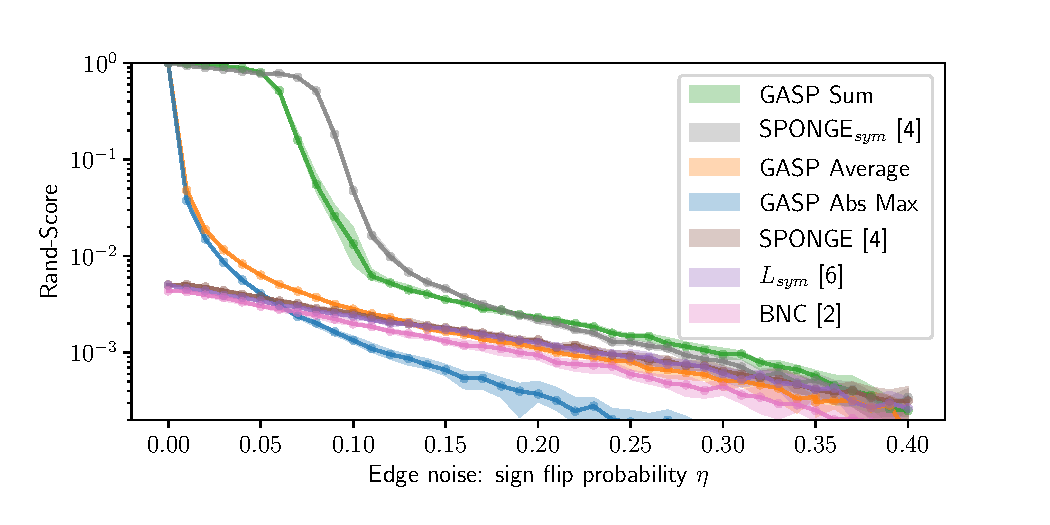
\includegraphics[width=1.\textwidth,trim=0.25in 0.25in 0.68in 0.36in,clip]{./figs/SSBM_experiments.pdf} % 0.45
        \caption{\algname{} performances compared to spectral methods on synthetic graphs. The spectral methods were given the true number of clusters as input, in contrast to \algname{}.}
    \label{fig:SSBM_spectral_experiments}
\end{minipage}
\end{figure}


\section{Comparison with spectral clustering} \label{sec:spectral_clust}
In this section we compare \algname{} to spectral clustering (SC) methods for signed graphs both on synthetic graphs and real ones from neuron segmentation. These methods require the user to specify the number of clusters in advance, in contrast to our proposed agglomeration method that determines the cluster number based on the signed weights of the graph. In the following comparison, we make these baselines as strong as possible by specifying the true number of clusters for the spectral methods.

\textbf{Synthetic graphs} -- First, we compare the clustering performance on synthetic graphs generated by a signed stochastic block model (SSBM), where SC performs well. In particular, we used an Erd\H os-R\'enyi random graph model $\mathcal{G}(N,p)$ with $N=10^5$ vertices and edge probability $p=0.1$. Following the approach in \cite{Cucuringu2019SPONGEAG}, we partitioned the graph into $k=100$ equally-sized clusters, such that edges connecting vertices belonging to the same cluster (different clusters, respectively) had Gaussian distributed edge weights centered at $\mu=1$ ($\mu=-1$, respectively) and with standard deviation $0.1$. To model noise, we flipped the sign of each edge independently with probability $\eta \in [0, 0.4]$. Median scores, 25th and 75th percentiles over 30 repetitions are shown in Fig.~\ref{fig:SSBM_spectral_experiments}: GASP achieved scores comparable to SPONGE$_{sym}$ \cite{Cucuringu2019SPONGEAG}, a recently proposed SC method. The specific design choice of a \emph{sign flipping} noise used in the SSBM experiments turned out to favor GASP with \emph{Sum} linkage that, according to the experiments presented in Sec.~\ref{sec:results}, is the one with the lowest tendency to over-cluster and grows one cluster at the time.

\textbf{Neuron segmentation} -- We extended the comparison with spectral methods to the task of neuron segmentation. Since SC cannot scale to the full CREMI dataset, we evaluated \algname{} and SC on a smaller $10\times100\times100$ voxels volume resulting in a graph with $10^5$ nodes and~$\sim10^6$ edges. Scores are summarized in Table \ref{tab:cremi_spectral_experiments}.
%suggested by the reviewer that performed best in the recent comparison \cite{Cucuringu2019SPONGEAG}: one based on the Balanced Normalized Cut (BNC) \cite{chiang2012scalable}; another on the symmetrically normalized Signed Laplacian ($L_{sym}$) \cite{kunegis2010spectral}; SPONGE and SPONGE$_{sym}$ algorithms were recently proposed in \cite{Cucuringu2019SPONGEAG}.
Despite the fact that the true number of ground truth clusters was given as an input to the SC methods, GASP significantly outperformed them on neuro-data. SC methods seem to have more difficulties when the graph is sparse. Moreover, they did not handle well pixels on the boundaries between segments and tended to cluster them together. Increasing $k$ did not improve their scores either.




% !TEX root = ../agglo_clust_review.tex
\section{Conclusion}
We have presented a unifying framework for agglomerative clustering of graphs with both positive and negative edge weights; and we have shown that some existing clustering algorithms, e.g. the Mutex Watershed, can be reformulated as special cases of this framework. 
We have analyzed several theoretical and empirical properties of the algorithms included in this framework. On instance segmentation, algorithms based on an average linkage criterion outperformed all the others: they proved to be simple and remarkably robust approaches to process short- and long-range predictions of a CNN.
 % applied to an instance segmentation task.
On biological images, these simple average agglomeration algorithms achieve state-of-the-art results without requiring the user to spend much time tuning complex task-dependent pipelines based on super-pixels.
% can represent a valuable choice for a user who is not willing to spend much time tuning complex task-dependent pipelines based on super-pixels.  
% In future work, we plan to explore common theoretical properties of the algorithms included in the framework.
% On biological images, this simple average agglomeration algorithm superpixels


{\small
\bibliographystyle{ieee_fullname}
\bibliography{agglo_clust}
}

\clearpage
% !TEX root = ../agglo_clust_review.tex

\section{Supplementary material}

\begin{algorithm}
  \caption{Implementation of \algname{}, generalized algorithm for signed graph partitioning}
\hspace*{\algorithmicindent} \textbf{Input:} $\mathcal{G}(V,E,w^+,w^-)$ with $N$ nodes and $M$ edges; boolean \texttt{{\color{blue}addCannotLinkConstraints}} \\
\hspace*{\algorithmicindent} \textbf{Output:} Final clustering \\
  \hspace*{\algorithmicindent} 
  \begin{algorithmic}[1]
    % \Procedure{GraphEdgeContr}{{\color{blue}bool \emph{addConstraints}}}
      % \State $\mathcal{G}'\gets \mathcal{G}(V,E^+ \cup E^-)$ \Comment{Initialize the contracted graph}
      \State $\tilde{\mathcal{G}}(\tilde{V},\tilde{E}) \gets \mathcal{G}(V,E,w^+,w^-)$  \Comment{Init. contracted graph}
      \State \texttt{UF} $\gets$ initUnionFind($V$) \Comment{Init. data structure representing clustering}
    %   \State PQ $\gets$ Sort $e\in E$ in descending order of $|w_e|$
        \State PQ.push$(|w_e|, e) \quad \forall e \in E $  \Comment{Init. priority queue in desc. order of $|w_e|=|w_e^+ - w_e^-|$, $\mathcal{O}(|E|)$}
        \State \texttt{canBeMerged}$[e] \gets$ \texttt{True} $\,\,\, \forall e\in E$ \Comment{Init. cannot-link constraints}
      % \State $E_\dagger \gets \{\}$ \Comment{Set of must-not-link edges}
    %   \State PQ.push$(e,  ) \quad \forall e \in E $  
    \State
      \While{PQ is \textbf{not} empty}
        \State $\tilde{w}, e_{uv} \gets $ PQ.popHighest() \Comment{$\mathcal{O}(\log |E|)$}
        \State \textbf{assert} \texttt{UF}.find($u$) $\neq$ \texttt{UF}.find($v$) \Comment{Edges in PQ always link nodes in different clusters}
        % \If{ $e_{uv} \notin E' $} 
        %     \State \textbf{continue}
        % \EndIf
        \If{({\color{ForestGreen}\textbf{$\tilde{w} > 0$}}) \textbf{and} \texttt{canBeMerged}$[e_{uv}]$}
        %   \State $u,v \gets u,v \in V' : $
        %   \State $S_u \gets S \in \Pi$ : $ u \in S$
        %   \State $S_v \gets S \in \Pi$ : $ v \in S$
          \State PQ, \texttt{canBeMerged}, $\tilde{E}$ $\gets$ \textsc{UpdateNeighbors}($u,v$)
        %   \State mergeDoubleEdges($u,v$) \Comment{Update PQ, $E_\dagger, \mathcal{G}'$}
          
        %   \State Update costs of double edges;
        %   \State Propagate constrained flags of double edges;
          \State $\tilde{V} \gets \tilde{V} \setminus \{ v\}$, $\quad \tilde{E} \gets \tilde{E} \setminus \{ e_{uv}\}$ \Comment{Update contracted graph}
        %   \State $ S_u \gets S_u \cup S_v$
          \State \texttt{UF}.merge($u,v$) \Comment{Merge clusters, $\mathcal{O}(\alpha(|E|))$}
          % \For{every new double edge}
          %   \State Delete double edges
          %   \State Insert new one with updated cost
          % \EndFor
        \ElsIf{({\color{red}\textbf{$\tilde{\cost} \leq 0$}}) \textbf{and} {\color{blue}\texttt{addCannotLinkConstraints}}}
          \State \texttt{canBeMerged}$[e_{uv}] \gets$ \texttt{False} \Comment{Constrain the two clusters}
        \EndIf
      \EndWhile
      \State
    %   \State
      \Return Final clustering given by union-find data structure  \texttt{UF}
      % \State
    % \EndProcedure
  \end{algorithmic}
  \hspace*{1.5cm} 
    \begin{algorithmic}[1]
    \Function{UpdateNeighbors}{$u,v$}
      % \State $\mathcal{G}'\gets \mathcal{G}(V,E^+ \cup E^-)$ \Comment{Initialize the contracted graph}
      \State $\mathcal{N}_u = \{ t \in \tilde{V} | e_{ut}\in \tilde{E}  \}$
      \State $\mathcal{N}_v = \{ t \in \tilde{V} | e_{vt}\in \tilde{E}  \}$ 
      \For{$t \in \mathcal{N}_v$ } \Comment{Loop over neighbors in $\tilde{\mathcal{G}}$ of deleted node $v$}
        \State $\tilde{E} \gets \tilde{E} \setminus \{e_{vt}\}$
        \State $\tilde{w}_{vt} \gets$ PQ.delete($e_{vt}$) \Comment{$\mathcal{O}(\log |E|)$}
        \State \texttt{canBeMerged}$[e_{ut}] \gets$ \texttt{canBeMerged}$[e_{ut}]$ \textbf{and} \texttt{canBeMerged}$[e_{vt}]$
        \If{$t \in \mathcal{N}_u$ }\Comment{$t$ is a common neighbor of $u$ and $v$}
          \State $\tilde{w}_{ut} \gets$ PQ.delete($e_{ut}$)  \Comment{$\mathcal{O}(\log |E|)$}
          \State PQ.push($ |f(\tilde{w}_{ut}, \tilde{w}_{vt})|, e_{ut}$) \Comment{$\mathcal{O}(\log |E|)$  }
        % \EndIf
        \Else
          \State $\tilde{E} \gets \tilde{E} \cup \{e_{ut}\}$
          \State PQ.push($ |\tilde{w}_{vt}|, e_{ut}$) \Comment{$\mathcal{O}(\log |E|)$}
        \EndIf
      \EndFor
      \State
    %   \State
      \Return PQ, \texttt{canBeMerged}, $\tilde{E}$
    %   % \State
    \EndFunction
  \end{algorithmic}
  \label{detailed_alg}
  % \caption{where $\alpha$ is the slowly growing inverse Ackerman function}
\end{algorithm}
\begin{figure}
        \centering
\begin{minipage}{0.49\textwidth}
\centering
        % 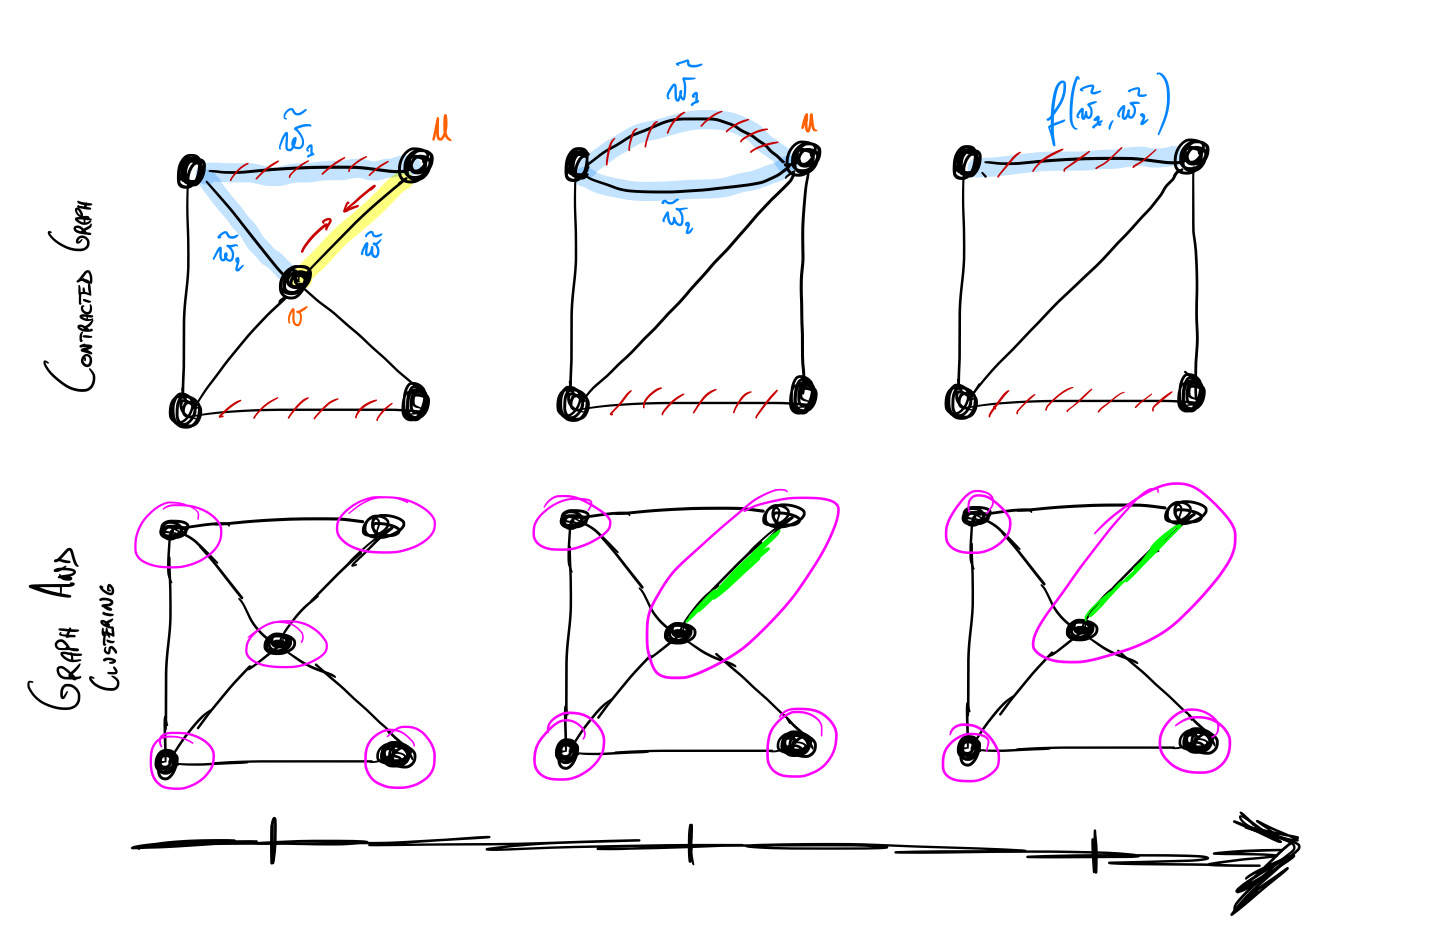
\includegraphics[width=\textwidth,trim=0.1in 0.4in 0.2in 0.2in,clip]{./figs/edge_contraction.png} % left bottom right top
        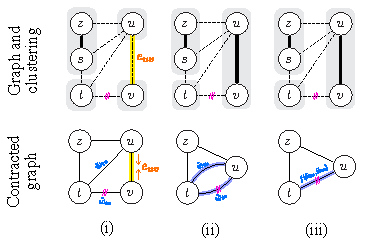
\includegraphics[width=\textwidth]{./figs/edge_contraction.pdf} % left bottom right top
% \captionof{figure}{ 
% {\small Example of edge contraction. First row: original graph $\mathcal{G}$; clustering $\Pi$ (gray shaded areas) with dashed edges on cut; cannot-link constraints (violet bars). Second row: contracted graph $\tilde{\mathcal{G}}_\Pi$. In step ii), edge $e_{uv}$ is contracted and node $v$ deleted from $\tilde{\mathcal{G}}_\Pi$. In step iii), double edges $e_{tu}$ and $e_{tv}$ resulting from edge contraction are replaced by single edge with updated interaction $f(\tilde{\cost}(e_{tu}), \tilde{\cost}(e_{tv}))$, see definitions in Tab.~\ref{tab:linkage-criteria}. }
% \label{fig:edge_contraction_and_contr_graph}  }
    \end{minipage} \hfill
\begin{minipage}[T]{0.48\textwidth}
    \centering
    \scriptsize
                \begin{tabular}[b]{r | l }
            \toprule
            % \multicolumn{2}{c||}{}  &   & \multicolumn{2}{c}{\textbf{Signed graphs}}  \\        
            % \cmidrule(l{.15em}){4-5}
            % \cline{4-5}
            % \multicolumn{2}{c||}{} & \textbf{Unsigned graphs} &  \multicolumn{2}{c}{\thead{Add Cannot-Link Constraints:}} \\        
            Linkage criteria & Update rule $f$ \\        
            \midrule
            Sum: & \thead[l]{$f(\tilde{\cost}_1,\tilde{\cost}_2) = \tilde{\cost}_1+\tilde{\cost}_2$} \\ 
            \makecell[r]{Absolute \\Maximum:} & \thead[l]{
            $
            f(\tilde{\cost}_1,\tilde{\cost}_2) = \begin{cases} 
            \tilde{\cost}_1 & \text{if}\,\, |\tilde{\cost}_1|>|\tilde{\cost}_2|\\
            \tilde{\cost}_2 & \text{otherwise}
             \end{cases} 
            $}
               \\ 
            \makecell[r]{Average:} & \thead[l]{$f(\tilde{\cost}_1,\tilde{\cost}_2) = \mathrm{weightAvg}\{ \tilde{\cost}_1, \tilde{\cost}_2 \} $}                 \\ 
            Maximum: & \thead[l]{$f(\tilde{\cost}_1,\tilde{\cost}_2) = \max \{ \tilde{\cost}_1, \tilde{\cost}_2 \}  $} \\
            Minimum:& \thead[l]{$f(\tilde{\cost}_1,\tilde{\cost}_2) = \min \{ \tilde{\cost}_1, \tilde{\cost}_2 \}  $} 
        \end{tabular}
    % \captionof{table}{}
    % \label{tab:linkage_and_update_rules}
\end{minipage}
\caption{ 
\textbf{Left:} Example of edge contraction. First row: original graph $\mathcal{G}$; clustering $\Pi$ (gray shaded areas) with dashed edges on cut; cannot-link constraints (violet bars). Second row: contracted graph $\tilde{\mathcal{G}}_\Pi$. In step ii), edge $e_{uv}$ is contracted and node $v$ deleted from $\tilde{\mathcal{G}}_\Pi$. In step iii), double edges $e_{tu}$ and $e_{tv}$ resulting from the edge contraction are replaced by a single edge with updated interaction. \textbf{Right:} The table lists the update rules $f(\tilde{\cost}_1, \tilde{\cost}_2)$ associated to the linkage criteria of Table \ref{tab:linkage-criteria} and that are used to efficiently update the interactions between clusters.}
\label{fig:edge_contraction_and_contr_graph}  
\end{figure}



\subsection{Implementation details and complexity of \algname{}} \label{sec:detailed_impl}


% During the agglomerative process, the interaction between adjacent clusters has to be properly updated and recomputed.  % given by the linkage criterion defined in Sec. \ref{sec:notation} and
% Given a graph $\mathcal{G}(V,E,\cost)$ and a clustering $\Pi$, we define the \emph{contracted graph} $\tilde{\mathcal{G}}_\Pi(\tilde{V}, \tilde{E}, \tilde{\cost})$, with $\tilde{V} \subseteq V$ such that node $u\in \tilde{V}$ represents the associated cluster $S_u \in \Pi$. Edges in $\tilde{E}$ are defined by adjacency-relationships between clusters and edge weights $\tilde{\cost}_{uv}$ represent inter-cluster interactions $\interact(S_u,S_v)$. 
\paragraph*{Update rules} During the agglomerative process, the interaction between adjacent clusters has to be properly updated and recomputed, as shown in Algorithm \ref{main_alg}.  % given by the linkage criterion defined in Sec. \ref{sec:notation} and
An efficient way of implementing these updates can be achieved by representing the agglomeration as a sequence of \emph{edge contractions} in the graph. Given a graph $\mathcal{G}(V,E,\cost)$ and a clustering $\Pi$, we define the associated \emph{contracted graph} $\tilde{\mathcal{G}}_\Pi(\tilde{V}, \tilde{E}, \tilde{\cost})$, such that there exists exactly one representative $|\tilde{V} \cap S| = 1$ for every cluster $S \in \Pi$ . Edges in $\tilde{E}$ represent adjacency-relationships between clusters 
and the signed edge weights $\tilde{\cost}_e$ are given by inter-cluster interactions $\tilde{\cost}(e_{uv})=\interact_{S_u,S_v}$. 
For the linkage criteria tested in this work, when two clusters $S_u$ and $S_v$ are merged, the interactions between the new cluster $S_u \cup S_v$ and each of its neighbors depend only on the previous interactions involving $S_u$ and $S_v$. Thus, we can recompute these interactions by using an \emph{update rule} $f$ that does not involve any loop over the edges of the original graph $\mathcal{G}$:
\begin{equation}
  \interact(S_u \cup S_v,S_t) = f\Big[ \interact(S_u,S_t), \interact(S_v,S_t) \Big] = f(\tilde{\cost}(e_{ut}), \tilde{\cost}(e_{vt})) %= \max \{ \tilde{\cost}(e_{ut}), \tilde{\cost}(e_{vt}) \}
\end{equation}
In Fig. \ref{fig:edge_contraction_and_contr_graph} we show an example of edge contraction and we list the update rules associated to the linkage criteria we introduced in Table \ref{tab:linkage-criteria}.
  % As an example, given the single-linkage criterion defined in Table , the interaction between $S_u \cup S_v$ and one of its neighbors $S_t$ is simply given by:
% All the update rules tested in this article are listed in Table \ref{tab:linkage-criteria}.

% \algname{} was implemented by using a standard agglomerative clustering algorithm based on a priority queue and a union
\paragraph{Implementation} As we show in Algorithm \ref{detailed_alg}, our implementation of \algname{} is based on an union-find data structure and a heap allowing deletion of its elements. The algorithm starts with each node assigned to its own cluster and sorts all edges $e\in E$ in a heap/priority queue (PQ) by their absolute weight $|\cost_e|=|w_e^+ - w_e^-|$ in descending order, so that the most attractive and the most repulsive interactions are processed first. It then iteratively pops one edge $e_{uv}$ from PQ and, depending on the priority $\tilde{\cost}_{uv}$, does the following: in case of attractive interaction $\tilde{\cost}_{uv}>0$, provided that $e_{uv}$ was not flagged as a cannot-link constraint, then merge the connected clusters, perform an edge contraction of $e_{uv}$ in $\tilde{\mathcal{G}}_\Pi$ and update the priorities of new double edges as explained in Fig. \ref{fig:edge_contraction_and_contr_graph}. 
% For every new pair of double edges in $\tilde{\mathcal{G}}_\Pi$, update their priorities according to one of the update rules listed in Table \ref{tab:linkage-criteria} together with their cannot-link relationships. 
If, on the other hand, the interaction is repulsive ($\tilde{\cost}_{uv}\leq 0$) and the option \texttt{addCannotLinkContraints} of Alg. \ref{detailed_alg} is \texttt{True}, then the edge $e_{uv}$ is flagged as cannot-link constraint.

\paragraph*{Complexity} In the main loop, the algorithm iterates over all edges, but the only iterations presenting a complexity different from $\mathcal{O}(1)$ are the ones involving a merge of two clusters, which are at most $N-1$. By using a union-find data structure (with path compression and union by rank) the time complexity of \texttt{merge}$(u, v)$ and \texttt{find}($u$) operations is $\mathcal{O}(\alpha(N))$, where $\alpha$ is the slowly growing inverse Ackerman function. The algorithm then iterates over the neighbors of the merged cluster (at most $N$) and updates/deletes values in the priority queue ($\mathcal{O}(\log |E|)$). Therefore, similarly to a heap-based implementation of hierarchical agglomerative clustering, our implementation of \algname{} has a complexity of $\mathcal{O}(N^2 \log N)$. In the worst case, when the graph is dense and $|E|=N^2$, the algorithm requires $\mathcal{O}(N^2)$ memory. Nevertheless, in our practical applications the graph is much sparser, so $\mathcal{O}(|E|)=\mathcal{O}(N)$. 
% and \UPDATE{in Fig. \ref{fig:runtime_plot} we show how the empirical runtime of \algname{} is much closer to $\mathcal{O}(N \log N)$ than $\mathcal{O}(N^2 \log N)$.} 
With a single-linkage, corresponding to the choice of the \emph{Maximum} update rule in our framework, the algorithm can be clearly implemented by using the more efficient Kruskal's Minimum Spanning Tree algorithm with complexity $\mathcal{O}(N \log N)$. 
Moreover, in the next section, we present an efficient implementation of \algname{} with \emph{Absolute Maximum} linkage that has empirical $\mathcal{O}(N \log N)$ complexity. %\TODO{Empirical complexity plot?}


\begin{algorithm}
  \caption{Mutex Watershed Algorithm proposed by \cite{wolf2018mutex}}
\hspace*{\algorithmicindent} \textbf{Input:} $\mathcal{G}(V,E,w^+,w^-)$ with $N$ nodes and $M$ edges \\
\hspace*{\algorithmicindent} \textbf{Output:} Final clustering \\
  \hspace*{\algorithmicindent} 
  \begin{algorithmic}[1]
      \State \texttt{UF} $\gets$ initUnionFind($V$) 
      % \State
      \For{$(u,v)=e\in E$ in descending order of $|w_e|=|w_e^+ - w_e^-|$}
        \If{\texttt{UF}.find($u$) $\neq$ \texttt{UF}.find($v$)} \Comment{Check if $u,v$ are already in the same cluster}
          \If{({\color{ForestGreen}\textbf{$w_e > 0$}}) \textbf{and} \texttt{canBeMerged}($u,v$)}  \Comment{Check for cannot-link constraints}
            \State \texttt{UF}.merge($u,v$) and inherit constraints of parent clusters
          \ElsIf{({\color{red}\textbf{$w_e \leq 0$}})}
            \State Add cannot-link constraints between parent clusters of $u,v$
          \EndIf
        \EndIf
      \EndFor
      \State
    %   \State
      \Return Final clustering given by union-find data structure \texttt{UF}
      % \State
    % \EndProcedure
  \end{algorithmic}
  \label{alg:mutex_watershed}
  % \caption{where $\alpha$ is the slowly growing inverse Ackerman function}
\end{algorithm}



\subsection{Properties of \algname{} with \emph{Absolute Maximum} linkage}\label{sec:appendix_abs_max}
\paragraph{Remark on graph notation} The definition of a graph proposed by \cite{wolf2018mutex} makes a distinction between a set of positive edges $E^+$, associated with a set $W^+$ of positive scalar attributes representing merge affinities, and a set of negative edges $E^-$, associated with a set $W^-$ of positive attributes representing split tendencies. On the other hand, in our definition $\mathcal{G}(V,E,w^+,w^-)$ each edge have both an attractive $w_e^+$ and a repulsive $w_e^-$ attribute, so we can make them equivalent by defining:
\begin{align}
E^+ = \{ e \in E \,\,\text{s.t.} \,\,w_e = w_e^+ - w_e^- > 0\},& \qquad E^- = \{ e \in E \,\,\text{s.t.}\,\, w_e = w_e^+ - w_e^- \leq 0\} \\
W^+ = \{ |w_e| \,\,\text{s.t.}\,\, e \in E^+\},& \qquad W^- = \{ |w_e| \,\,\text{s.t.}\,\, e \in E^-\}
\end{align}

\begin{prop} \label{prop:equiv_MWS}
The Mutex Watershed Algorithm \ref{alg:mutex_watershed} (MWS) with empirical $\mathcal{O}(N \log N)$ complexity introduced by \cite{wolf2018mutex} returns the same final clustering given by the \algname{} Algorithm \ref{detailed_alg} with the use of cannot-link constraints and an Absolute Maximum update rule:
\begin{equation}\label{eq:def_abs_max}
f_{\mathrm{Abs.Max.}}(\tilde{\cost}_1,\tilde{\cost}_2) = \begin{cases} 
            \tilde{\cost}_1 & \text{if}\,\, |\tilde{\cost}_1|>|\tilde{\cost}_2|\\
            \tilde{\cost}_2 & \text{otherwise}
             \end{cases} 
\end{equation}
\end{prop}
\begin{proof}
Both algorithms sort edges in descending order of the absolute interactions $|w_e|$ and then iterate over all of them. The only difference is that MWS, after merging two clusters, does not update the interactions between the new cluster and its neighbors. 
However, since with an Abs. Max. linkage the interaction between clusters is simply given by the edge with highest absolute weight $|w_e|$, the order by which edges are iterated over in \algname{} is never updated. Thus, both algorithms perform precisely the same steps and return the same clustering.
\end{proof}
\begin{prop}
The \algname{} Algorithm \ref{detailed_alg} with the Absolute Maximum linkage defined in Eq. \ref{eq:def_abs_max} returns the same final clustering whether or not cannot-link constraints are enforced. 
\end{prop}
\begin{proof}
% In Proposition \ref{prop:equiv_MWS} we observed that \algname{} with Abs. Max. linkage never updates the order by which edges are iterated over
In the \algname{} Algorithm \ref{detailed_alg}, the clustering is updated only when two clusters are merged and the condition at line 9 is satisfied. 
We also observe that, in the unconstrained version of \algname{}, the predicate \texttt{canBeMerged} at line 9 can never be false because cannot-link constraints are never introduced at line 14.
Let us now contradict the initial hypothesis and assume by absurd that the constrained version of \algname{} introduces a cannot-link constraints between two clusters sharing a positive interaction $\tilde{w}>0$ and outputs a different clustering as compared to the unconstrained version. 
This can happen only in the situation shown in Fig. \ref{fig:abs_max_proof_example}, when two clusters $u$ and $v$ are merged together and share a common neighboring node $t$ having the following two properties: a) $u$ and $t$ are already constrained and share a repulsive interaction $w_{ut}\leq0$, b) $v$ and $t$ share an attractive interaction $w_{vt}>0$ that is higher in absolute value $|w_{vt}|>|w_{ut}|$. 
Then, according to Eq. \ref{eq:def_abs_max}, the new merged cluster $uv$ and $t$ are constrained and share a positive interaction. 
But this case can never happen, since if $|w_{vt}|>|w_{ut}|$ then clusters $v$ and $t$ are merged before clusters $u$ and $t$ are constrained.  
\end{proof}


\begin{figure}
        \centering

        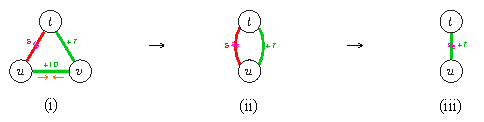
\includegraphics[width=0.7\textwidth]{./figs/proof_abs_max_example.pdf} % left bottom right top
\caption{\algname{} with \emph{AbsMax} linkage: Example representing the only case of edge contraction $e_{uv}$ that would introduce a positive attractive interaction between two constrained clusters. Note this can actually never happen with an \emph{AbsMax} linkage, because edge $e_{ut}$ has a lower absolute priority as compared to $e_{uv}$, so clusters $u$ and $t$ cannot have been constrained before $u$ and $v$ are merged.
}
\label{fig:abs_max_proof_example}  
\end{figure}




% \subsection{Multicut and correlation clustering } 
% \TODO{Omit completely?} For any clustering $\Pi$ of $\mathcal{G}$, we define as $E^{\mathrm{internal}}_\Pi$ the set of edges linking nodes in the same cluster, and as $E_\Pi^{\mathrm{external}}$ the complementary set of edges whose incident nodes belong to distinct clusters:
% \begin{equation}
% E_\Pi^{\mathrm{internal}} \equiv \{ e_{uv} \in E \,|\, \exists S \in \Pi : u \in S \, \text{and} \, v \in S \}, \qquad E^{\mathrm{external}}_\Pi \equiv E \setminus E^{\mathrm{internal}}_\Pi.
% \end{equation}
% % \begin{align}
% % E_\Pi^0 &= \{ e_{uv} \in E \,|\, \exists S \in \Pi : u \in S \, \text{and} \, v \in S \}, \\
% % E^1_\Pi &= E \setminus E^0_\Pi.
% % \end{align}
% The set of edges $E_\Pi^{\mathrm{external}}$ is known as the \emph{multicut} of $\mathcal{G}$ w.r.t. clustering $\Pi$. The instance of the NP-hard \emph{weighted correlation clustering/multicut problem} 
% % w.r.t. $\mathcal{G}(V,E,\cost)$ 
% corresponds to finding the partitioning that optimally balance attraction and repulsion in the graph and is given by the following binary integer program \cite{kappes2011globally,chopra1991multiway,andres2015lifting}:
% \begin{equation}\label{eq:multicut_obj}
% % \min_\Pi \texttt{MC}(\Pi) \equiv
%  \min_\Pi \sum_{e\in E} \cost_e x_e^\Pi,  \qquad \text{where} \quad x^\Pi_e = 
%  \begin{cases} 
%  1 & \text{if } e\in E^{\mathrm{external}}_\Pi \\
%  0 & \text{otherwise}.
%  \end{cases}
% \end{equation}
% In the next chapters we will use this objective as measure of how balanced a clustering is.

\subsection{Predicting signed edge weights with a CNN}
Our CNN model outputs affinities in the form of pseudo-probabilities $p:E \rightarrow [0,1]$, where $p=0$ represents a boundary evidence. In order to use them as input of the algorithms in our framework, we mapped them to positive and negative values\footnote{Note that in general attractive and repulsive interactions $w^+$ and $w^-$ can be independently estimated with different classifiers.}. The most common approaches use \emph{additive} \cite{ailon2008aggregating} or \emph{logarithmic} \cite{finkel2008enforcing,andres2012globally} mappings:
\begin{equation} \label{eq:mappings}
\cost_{e,\mathrm{Add}} = p_e - \beta, \qquad \quad \cost_{e,\mathrm{Log}} = \log \left( \frac{p_e}{1-p_e} \right) - \log \left( \frac{\beta}{1-\beta} \right),
\end{equation}
where $\beta \in [0,1]$ is a \emph{bias} parameter that allow a tuning between over- and under-segmentation. We evaluated both of them empirically with each of the tested linkage and found that the additive mapping is the best option in all cases apart from the \emph{Sum} linkage. Note that varying the parameter $\beta$ does not usually define a hierarchy of nested clusterings, thus it is not equivalent to varying a threshold parameter in HAC. This hierarchical property is only valid for \algname{} without constraints and with \emph{Average}, \emph{Max} or \emph{Min} linkage.



\subsection{Neuron segmentation and compared methods}\label{sec:cremi_details}
\paragraph{Training details} The data from the CREMI challenge is highly anisotropic and contains artifacts like missing sections, staining precipitations and support film folds. 
To alleviate difficulties stemming from misalignment, we use a version of the data that was elastically realigned by the challenge organizers with the method of \cite{saalfeld2012elastic}.
We train a 3D U-Net \cite{ronneberger2015u, cciccek20163d} using the same architecture as \cite{funke2018large} and predict long-and-short range affinities 
as described in \cite{lee2017superhuman}. In addition to the standard data augmentation techniques of random rotations, random flips and  elastic deformations, we simulate data artifacts.
In more detail, we randomly zero-out slices, decrease the contrast of slices, simulate tears, introduce alignment jitter and paste artifacts extracted from the training data. Both \cite{funke2018large} and \cite{lee2017superhuman} have shown
that these kinds of augmentations can help to alleviate issues caused by EM-imaging artifacts.
We use L2 loss and Adam optimizer to train the network. The model was trained on all the three samples with available ground truth labels.  

\paragraph{THRESH and WSDT} The basic post-processing methods we consider cannot take long-range affinities into account, so we only consider direct neighbors affinities and generate a boundary map by taking an average over the 3 directions. Based on this boundary map, we run connected components (THRESH) and we also introduce seeds at the maxima of the smoothed distance transform (WSDT). For WSDT, the degree of smoothing was optimized such that each region receives as few seeds as possible, without however causing severe under-segmentation. Due to the anisotropy of the data, we generate 2D WSDT superpixels by considering each 2D image in the stack singularly.


\paragraph{Multi-step pipelines} Given the 2D WSDT superpixels, we build a 3D region-adjacency graph such that each node represents a superpixel. The weights of the edges connecting neighboring superpixels are computed by taking an average over both short- and long-range affinities connecting the two regions. We then convert the edge probabilities to signed weights using the logarithmic mapping defined in Eq. \ref{eq:mappings} and solve the multicut problem on this graph. For our experiments, we use the approximate Kernighan-Lin solver \cite{keuper2015efficient,kernighan1970efficient} (WSDT+MC). In some cases, the long-range affinities predicted by the CNN can connect two superpixels that are not direct-neighbors. Thus, in these cases we introduce additional \emph{lifted} edges in the graph and an instance of the lifted multicut problem (WSDT+LMC). This time, similarly to the methods mentioned in \cite{beier2016efficient}, we used a combination of approximate solvers consisting in GAEC and Kernighan-Lin. 
%and      Other state-of-the-art multi-step-pipelines for neuron-segmentation first find 2D superpixels using WSDT and then apply a graph partitioning algorithm: in our comparison, we include one pipeline using hierarchical agglomerative clustering with average linkage (avgHC) and one using an approximation of the Lifted Multicut Problem (LMC) \cite{beier2016efficient}.

\subsection{\algname{} on the full CREMI dataset} \label{sec:appendix_exps_full_cremi}
 \paragraph{Pre-merge processing} For the predictions on the full dataset from the CREMI challenge, we used  the padded volumes provided by the challenge. The crops on which we performed a prediction have a size of $1500\times1500\times127=2.86\cdot 10^8$ voxels or larger. Building a graph with $10^8$ nodes can easily incur a large use of memory, so we decided to perform a preprocessing step by initially merging some nodes together. Simply down-sampling the predictions of the CNN would have led to a loss of resolution and performances in the most difficult parts of the dataset. Thus, we decided to pre-merge the most connected components of the graph that would be anyway clustered during the first iterations of \algname{}. To do this, we used a simple approach: we generated a boundary probability map by taking for each voxel an average over affinities in all directions (both short- and long-range ones) and we run THRESH to find the connected components. With this approach, pixels are pre-clustered only when they are far away (in all directions) from all predicted boundaries. 
 To make sure that in this preprocessing step different neurons are never merged together by mistake, we intersected these segments given by the conservative THRESH with the segments given by WSDT. %\TODO{show figure?}
 By using this method, we initialized \algname{} with a reduced graph that represents a true over-segmentation. In our experiments, the use of this preprocessing method did not impact the final scores achieved by \algname{} and significantly reduced its runtime. On the full datasets, we used only 10 \% of the long-range connections in the pixel-graph, since adding all of them did not improve the scores and only made the simulations much slower and memory inefficient. 
 
 \paragraph{Removing small segments} After running \algname{}, we use a simple post-processing step to delete small segments on the boundaries, most of which are given by single-voxel clusters. On the neuron segmentation predictions, we deleted all regions with less than 200 voxels and used a seeded watershed algorithm to expand the bigger segments.

 \paragraph{Enforcing local merge} In 2D images of urban-scenes, due to partial occlusion, one object instance can be given by multiple components that are not directly connected in the image plane. This is not the case in neuron-segmentation, where each neuron should be given by a single 3D connected component in the volume. In order to enforce it, we modified the implementation of \algname{} so that two clusters are merged only when they represent two adjacent supervoxels in the 3D volume and if this condition is not satisfied, the merge is postponed until there is a direct connection. This then avoids the introduction of ``air-bridges'' between segments due to attractive long-range connections in the initial voxel grid-graph.
 This approach achieved superior performances to the one proposed in \cite{wolf2018mutex}, where all long-range connections in the grid-graph are associated to a negative repulsive edge weight.

\begin{table}[t]
\centering
    \footnotesize
% \begin{minipage}[T]{0.85\textwidth}
%     \centering
        \begin{tabular}{l|c|c|c|c|c}
          \algname{} linkage & \makecell{CREMI-Score\\(higher better)}  & \makecell{Rand-Score\\(higher better)} & \makecell{VI-merge\\(lower better)} & \makecell{VI-split\\(lower better)} & \makecell{Runtime\\(lower better)} \\ \midrule
          % Pipeline & method & \textsc{No} & \textsc{Yes} \\ 

% Average & 0.226 & 0.936 & 0.315 & 0.494 & 
% Sum + CLC & 0.282 & 0.906 & 0.358 & 0.510 & 
% Abs Max & 0.322 & 0.897 & 0.286 & 0.735 & 
% Max + CLC & 0.324 & 0.893 & 0.292 & 0.698 & 
% Sum & 0.334 & 0.872 & 0.461 & 0.444 & 
% Average + CLC & 0.563 & 0.772 & 0.259 & 1.142 & 
% Min & 2.522 & 0.030 & 0.197 & 6.365 & 
% Min + CLC & 2.522 & 0.030 & 0.197 & 6.365 & 
% Max & 2.626 & 0.028 & 7.069 & 0.026 & 
Average & \textbf{0.226} & \textbf{0.936} & 0.315 & 0.494 & 3.49 $\cdot$ 10$^4$ \\
Sum + CLC \cite{levinkov2017comparative} & 0.282 & 0.906 & 0.358 & 0.510 & 4.64 $\cdot$ 10$^4$ \\
Abs Max \cite{wolf2018mutex} & 0.322 & 0.897 & 0.286 & 0.735 & 1.24 $\cdot$ 10$^4$ \\
Max + CLC & 0.324 & 0.893 & 0.292 & 0.698 & 6.31 $\cdot$ 10$^4$ \\
Sum \cite{keuper2015efficient} & 0.334 & 0.872 & 0.461 & 0.444 & 4.74 $\cdot$ 10$^4$ \\
Average + CLC & 0.563 & 0.772 & 0.259  & 1.142 & 2.95 $\cdot$ 10$^4$ \\
Min & 2.522 & 0.030 & \textbf{0.197} & 6.365 & 2.97 $\cdot$ 10$^3$ \\
Min + CLC & 2.522 & 0.030 & \textbf{0.197}  & 6.365 & 4.77 $\cdot$ 10$^3$ \\
Max & 2.626 & 0.028 & 7.069 & \textbf{0.026} & \textbf{6.04 $\cdot$ 10$^\mathbf{2}$} \\
        \end{tabular}
        \vspace*{1.1em}
    \caption{Performances achieved by different versions of \algname{} on the CREMI 2016 training set. 
    CREMI-Score \cite{cremiChallenge}, is given by a combination of the Adapted Rand-Score (Rand-Score) and the Variation of Information Score for under-clustering (VI-merge) and over-clustering (VI-split) \cite{arganda2015crowdsourcing}.
    CLC stands for cannot-link constraints. For all algorithms, the chosen value of bias parameter was $\beta = 0$. We used a machine with CPU Intel(R) Xeon(R) X5650  @ 2.67GHz for our comparison experiments.}
    \label{tab:extended_results_cremi}
\end{table}
% \hfill
% \begin{minipage}[T]{0.6\textwidth}
% \centering
%         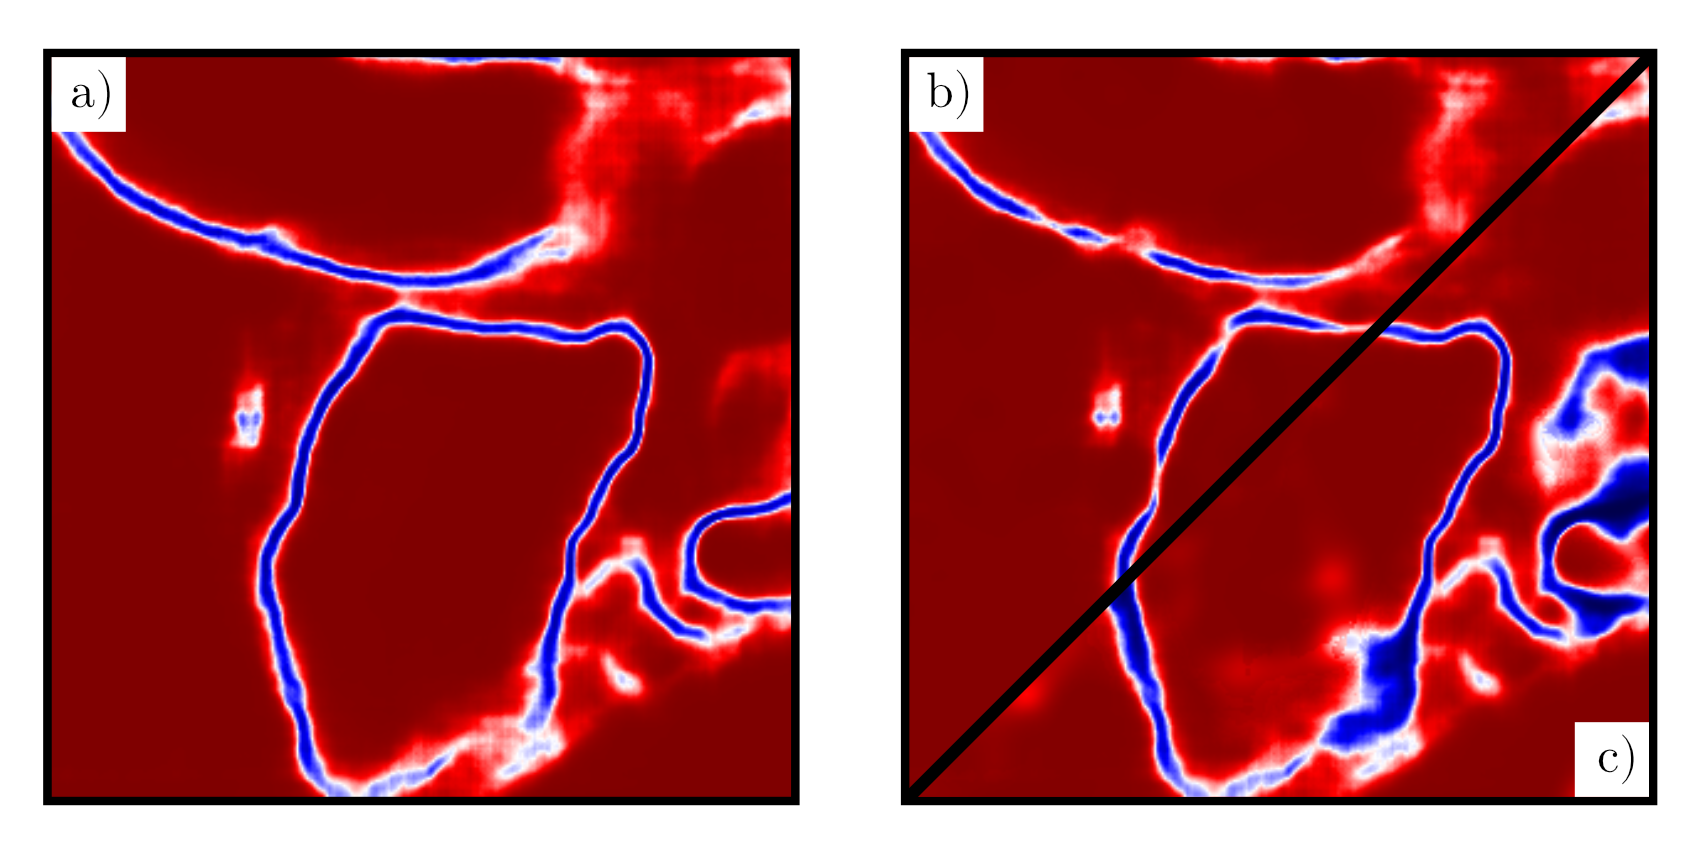
\includegraphics[width=0.88\textwidth,trim=0.1in 0.0in 0.05in 0.0in,clip]{figs/noisy_affs_comparison.png}
%     \captionof{figure}{The two figures represent the CNN predictions on a slice of the neuron segmentation CREMI challenge \cite{cremiChallenge} with and without additional noise. Blue pixels represent boundary evidence. Image a) shows the original CNN predictions, b) the merge-biased version $\tilde{F}_{+}$ and c) the split-biased version $\tilde{F}_{-}$ (see definition \ref{eq:noise_biased_predictions}). \TODO{Overlay raw-data}
%     %The color of each pixel represents how probable it is for it to be in the same cluster with its neighboring pixel on the right (red: same cluster; blue: different ones). 
%     %Adding merge-biased noise tends to create holes in the boundaries; split-biased noise add non-existing boundaries 
%     }
%     \label{fig:noisy_affs}
% \end{minipage}
% \end{figure}


\subsection{Experiments on neuron segmentation adding noise to CNN predictions} \label{sec:appendix_noise_gen}
Additionally to the comparison on the full training dataset, we performed additional experiments on a crop of the more challenging CREMI training sample B, where we perturbed the predictions of the CNN with noise and we introduced additional artifacts like missing or fictitious boundary evidences.
% Fig. \hyperref[fig:noisy_affs]{\ref*{fig:noisy_affs}a} shows an example of uncertain CNN predictions on a part of the neuron segmentation CREMI dataset. We now present a way of modifying the CNN output to introduce additional artifacts like a missing or false boundary evidence. 

In the field of image processing there are several ways of adding noise to an image, among which the most common are Gaussian noise or Poisson shot noise. 
In these cases, the noise of one pixel does not correlate with its neighboring noise values. On the other hand, predictions of a CNN are known to be spatially correlated. 
Thus, we used Perlin noise\footnote{In our experiments, we used an open-source implementation of simplex noise \cite{perlin2001noise}, which is an improved version of Perlin noise \cite{perlin1985image}}, one of the most common gradient noises used in procedural pattern generation. This type of noise $n(x)\in[0,1]$ generates spatial random patterns that are locally smooth but have large and diverse variations on bigger scales. We then combined it with the CNN predictions $p(x)$ in the two following ways: 
\begin{equation}\label{eq:noise_biased_predictions}
% \tilde{F}(x;\theta)=\begin{cases}
% F(x;\theta)+\mathcal{K}\cdot\max\left(N(x),0\right) & \text{if merge-biased}\\
% F(x;\theta)+\mathcal{K}\cdot\min\left(N(x),0\right) & \text{if split-biased}
% \end{cases}
\tilde{F}_{\pm}(x;\mathcal{K})=F(x)\pm\big|\mathcal{K}\cdot\max\left(\pm N(x),0\right)\big|,
\end{equation}
where  $N(x)=\mathrm{Logit}[n(x)]$; $F(x)=\mathrm{Logit}[p(x)]$ and $\mathcal{K}\in \mathbb{R}^+$ is a positive factor representing the amount of added noise. $\tilde{F}_{+}(x;\mathcal{K})$ represents then a under-clustering biased prediction, such that the probability for two pixels to be in the same cluster is increased only if $N(x)>0$ (see Fig. \hyperref[fig:noisy_affs]{\ref*{fig:noisy_affs}b}), whereas $\tilde{F}_{-}(x;\mathcal{K})$ is a over-clustering biased prediction with decreased probabilities when $N(x)<0$ (Fig. \hyperref[fig:noisy_affs]{\ref*{fig:noisy_affs}c}).
In the implementation we used, the noise can be generated in an arbitrary number of dimensions and a smoothing factor can be specified for each direction independently. In our experiments, each pixel is represented by a node in the grid-graph and it is linked to $n_{\mathrm{nb}}$ other nodes by short- and long-range edges. Thus, the output of our CNN model has $n_{\mathrm{nb}}$ channels: for each pixel / voxel, it outputs $n_{\mathrm{nb}}$ values representing the weights of different edge connections. We then generated a 4-dimensional noise that matches the dimension of the CNN output. The data is highly anisotropic, i.e. it has a lower resolution in one of the dimensions. Due to this fact, we chose different smoothing parameters to generate the noise in different directions. 

The experiments summarized in Fig. \ref{fig:noise_plots} were performed in the following way: for each value $\mathcal{K}$, 30 random noise samples were drawn, from which median and percentiles statistics were computed for each different linkage criteria. For each sample, we randomly selected some of the long-range predictions from the CNN and added them to pixel grid-graph.
% one of the dimensions has a lower resolution,   such that three dimensions represent the spatial ones a
% \multirow{2}{*}{Sum} &No & 0.55  & {\color{Orange} 0.313 } & {\color{Orange} 0.511 } \\
%  &Yes & 0.55  & {\color{Orange} 0.319 } & {\color{Orange} 0.527 } \\\midrule
% % Abs. max. &- & 0.45  & {\color{Orange} 0.321 } & {\color{ForestGreen} 0.531 } \\\midrule
% % \multirow{2}{*}{Mean} &No & 0.35  & {\color{ForestGreen} 0.343 } & {\color{ForestGreen} 0.552 } \\
%  % &Yes & 0.25  & {\color{Orange} 0.339 } & {\color{ForestGreen} 0.548 } \\\midrule
% \multirow{2}{*}{Max} &No & 0.85 & {\color{Red} 0.243 } & {\color{Red} 0.444 } \\
%  &Yes & 0.50  & {\color{Orange} 0.325 } & {\color{ForestGreen} 0.530 } \\\midrule
% \multirow{2}{*}{Min} &No & 0.50  & {\color{Red} 0.000 } & {\color{Red} 0.000 } \\
%  &Yes & 0.50  & {\color{Red} 0.000 } & {\color{Red} 0.000 } \\\midrule
% \cite{liu2018affinity} &-  & -  & {\color{ForestGreen} 0.341 } & {\color{ForestGreen} 0.547 } \\
\begin{figure}[t]
\centering
\begin{minipage}[T]{0.6\textwidth}
\centering
        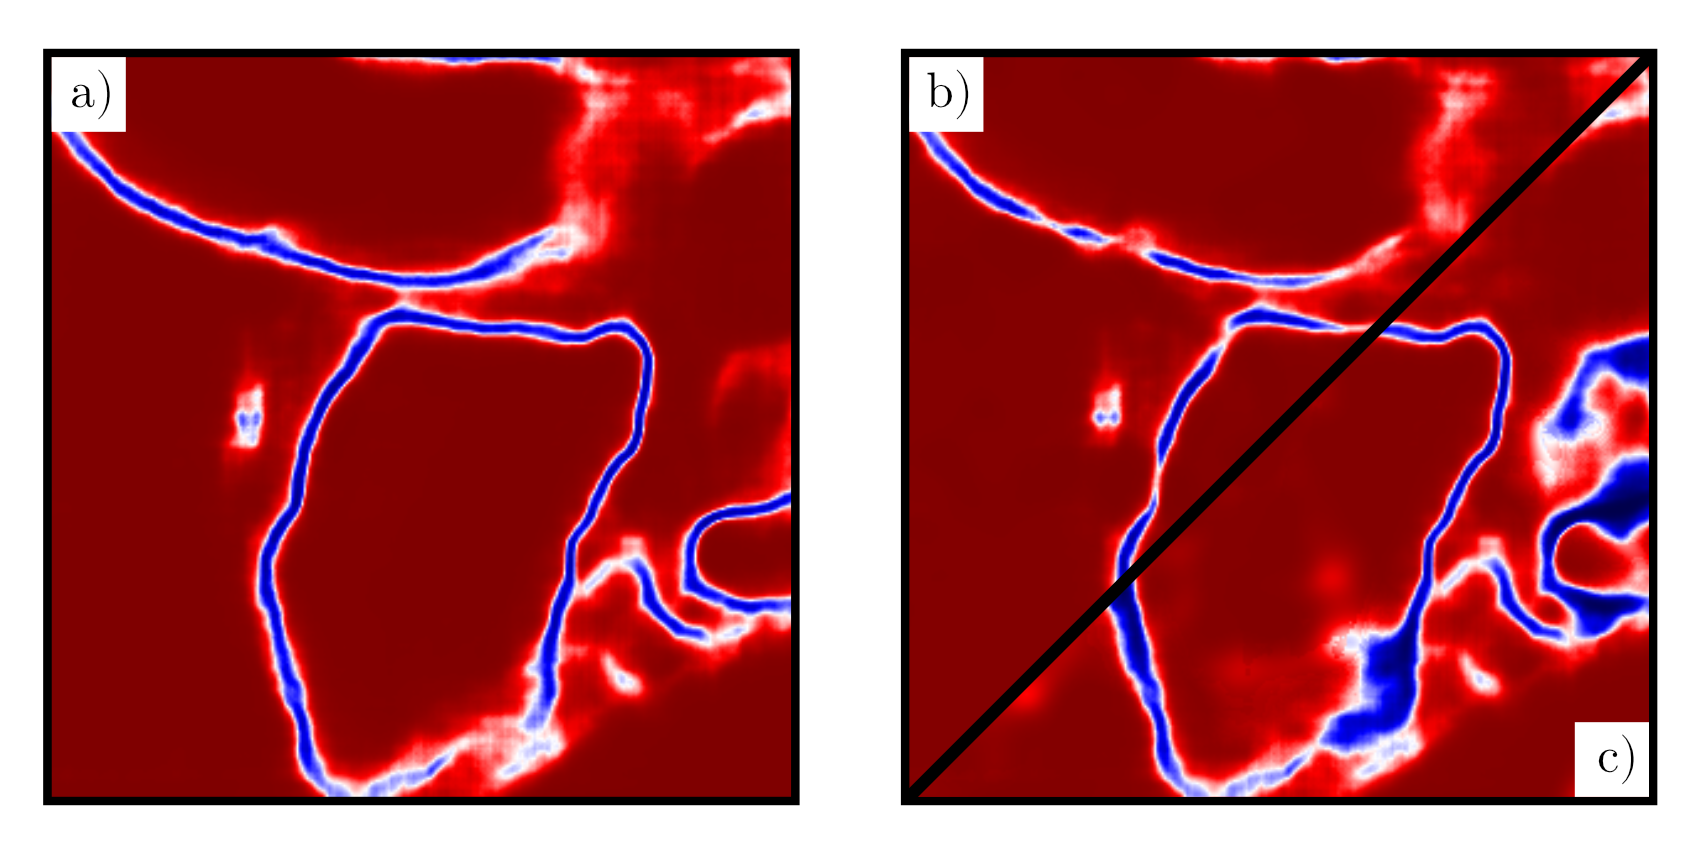
\includegraphics[width=0.88\textwidth,trim=0.1in 0.0in 0.05in 0.0in,clip]{figs/noisy_affs_comparison.png}
    \captionof{figure}{The two figures represent the CNN predictions on a slice of the neuron segmentation CREMI challenge \cite{cremiChallenge} with and without additional noise. Blue pixels represent boundary evidence. Image a) shows the original CNN predictions, b) the under-clustering biased version $\tilde{F}_{+}$ and c) the over-clustering biased version $\tilde{F}_{-}$ (see definition \ref{eq:noise_biased_predictions}). 
    %The color of each pixel represents how probable it is for it to be in the same cluster with its neighboring pixel on the right (red: same cluster; blue: different ones). 
    %Adding merge-biased noise tends to create holes in the boundaries; split-biased noise add non-existing boundaries 
    }
    \label{fig:noisy_affs}
\end{minipage}\hfill
\begin{minipage}[T]{0.35\textwidth}
    \centering
    \footnotesize
        \begin{tabular}{l|c|c}
          \algname{} linkage & AP  & Bias $\beta$ \\ \midrule
          % Pipeline & method & \textsc{No} & \textsc{Yes} \\ 
          Average & 34.3 & 0.35 \\
          Average + CLC & 33.9 & 0.25\\
          Max + CLC & 32.5 & 0.50 \\
          Abs Max & 32.1 & 0.45\\
          Sum + CLC & 31.9 & 0.55 \\
          Sum & 31.3 & 0.55 \\
          Max & 24.3 & 0.85 \\
          Min & 0.00 & 0.50 \\
          Min + CLC & 0.00 & 0.50 \\
        \end{tabular}
    \captionof{table}{Average Precision (AP) scores achieved by different versions of \algname{} and chosen bias parameters $\beta$ on the cityscapes validation set. A bias value $\beta=0$ returns one single cluster. CLC stands for cannot-link constraints}
    \label{tab:extended_results_cityscapes_val}
\end{minipage}
\end{figure}



\subsection{Fine-tuning the GMIS pipeline on CityScapes} \label{sec:appendix_cityscapes}
For our experiments, we used the model from GMIS \cite{liu2018affinity} that is publicly available. The instance-branch of the model was trained with a Binary Cross-Entropy loss, but we noticed how the short-range affinities were biased towards high probabilities, so that a strong short-range boundary evidence was never predicted by the model. In \cite{liu2018affinity}, they handle this problem by proposing a modified version of HAC that is done in stages (MultiStepHAC): initially only short-range affinities are used to run HAC and a low threshold in the hierarchy is chosen to define a first clustering; then a new HAC problem including long-range affinities is  initialized with the first clustering; in the method proposed by \cite{liu2018affinity}, these steps are repeated three times. 

Since MultiStepHAC is a rather complex post-processing method that requires to tune several hyper-parameters, we opted for a different approach to solve the problem of the unbalanced affinities. We added two 1x1 convolutional layers to the instance-branch model and trained them by using the same loss used for example by \cite{wolf2018mutex} and is based on the S\o resen-Dice coefficient \cite{dice1945measures,sorensen1948method}. Compared to Hamming-distance based loss like Binary Cross-Entropy or Mean Squared Error, the advantage of this loss is its being robust against prediction and / or target sparsity, that is a desirable quality in this application since boundaries between instances can be sparse. 
During training, all the affinities involving at least one pixel belonging to the background were ignored in the loss. In this way, these last two layers specialized in improving the predictions of boundary evidence between adjacent instances (especially those belonging to the same class). We then considered an average of these new fine-tuned affinities with the original unbalanced ones predicted by the model. During the fine-tuning process, only the parameters in the last two layers were updated.

Before to apply \algname{}, we performed a parameter-search for the bias $\beta$ defined in \ref{eq:mappings}. Table \ref{tab:extended_results_cityscapes_val} lists the best-case performances for each of the methods with the chosen bias $\beta$: note that depending on the version of \algname{}, it was necessary to bias more or less the predicted edge weights.




\section*{Divide and conquer}
\TODO{}
Who takes responsibility for what part? And make corrections / suggestions by what date?

Nathan: Appendix, by sunday

Constantin: 3.1, 3.2, Algorithm 1; by Monday evening
Steffen: I have also started working on the sections
         3.1, 3.2 Algorithm 1; 3.3 + Appendix;
         I will focus more on 3.3 + related Appendix A6.2 (pages 14-16)
         by Monday evening
    
\end{document}
